% Options for packages loaded elsewhere
\PassOptionsToPackage{unicode}{hyperref}
\PassOptionsToPackage{hyphens}{url}
\PassOptionsToPackage{dvipsnames,svgnames,x11names}{xcolor}
%
\documentclass[
  a4paper,
]{ltjsbook}

\usepackage{amsmath,amssymb}
\usepackage{iftex}
\ifPDFTeX
  \usepackage[T1]{fontenc}
  \usepackage[utf8]{inputenc}
  \usepackage{textcomp} % provide euro and other symbols
\else % if luatex or xetex
  \usepackage{unicode-math}
  \defaultfontfeatures{Scale=MatchLowercase}
  \defaultfontfeatures[\rmfamily]{Ligatures=TeX,Scale=1}
\fi
\usepackage{lmodern}
\ifPDFTeX\else  
    % xetex/luatex font selection
\fi
% Use upquote if available, for straight quotes in verbatim environments
\IfFileExists{upquote.sty}{\usepackage{upquote}}{}
\IfFileExists{microtype.sty}{% use microtype if available
  \usepackage[]{microtype}
  \UseMicrotypeSet[protrusion]{basicmath} % disable protrusion for tt fonts
}{}
\makeatletter
\@ifundefined{KOMAClassName}{% if non-KOMA class
  \IfFileExists{parskip.sty}{%
    \usepackage{parskip}
  }{% else
    \setlength{\parindent}{0pt}
    \setlength{\parskip}{6pt plus 2pt minus 1pt}}
}{% if KOMA class
  \KOMAoptions{parskip=half}}
\makeatother
\usepackage{xcolor}
\usepackage[top=30mm,left=20mm,heightrounded]{geometry}
\setlength{\emergencystretch}{3em} % prevent overfull lines
\setcounter{secnumdepth}{5}
% Make \paragraph and \subparagraph free-standing
\ifx\paragraph\undefined\else
  \let\oldparagraph\paragraph
  \renewcommand{\paragraph}[1]{\oldparagraph{#1}\mbox{}}
\fi
\ifx\subparagraph\undefined\else
  \let\oldsubparagraph\subparagraph
  \renewcommand{\subparagraph}[1]{\oldsubparagraph{#1}\mbox{}}
\fi

\usepackage{color}
\usepackage{fancyvrb}
\newcommand{\VerbBar}{|}
\newcommand{\VERB}{\Verb[commandchars=\\\{\}]}
\DefineVerbatimEnvironment{Highlighting}{Verbatim}{commandchars=\\\{\}}
% Add ',fontsize=\small' for more characters per line
\usepackage{framed}
\definecolor{shadecolor}{RGB}{241,243,245}
\newenvironment{Shaded}{\begin{snugshade}}{\end{snugshade}}
\newcommand{\AlertTok}[1]{\textcolor[rgb]{0.68,0.00,0.00}{#1}}
\newcommand{\AnnotationTok}[1]{\textcolor[rgb]{0.37,0.37,0.37}{#1}}
\newcommand{\AttributeTok}[1]{\textcolor[rgb]{0.40,0.45,0.13}{#1}}
\newcommand{\BaseNTok}[1]{\textcolor[rgb]{0.68,0.00,0.00}{#1}}
\newcommand{\BuiltInTok}[1]{\textcolor[rgb]{0.00,0.23,0.31}{#1}}
\newcommand{\CharTok}[1]{\textcolor[rgb]{0.13,0.47,0.30}{#1}}
\newcommand{\CommentTok}[1]{\textcolor[rgb]{0.37,0.37,0.37}{#1}}
\newcommand{\CommentVarTok}[1]{\textcolor[rgb]{0.37,0.37,0.37}{\textit{#1}}}
\newcommand{\ConstantTok}[1]{\textcolor[rgb]{0.56,0.35,0.01}{#1}}
\newcommand{\ControlFlowTok}[1]{\textcolor[rgb]{0.00,0.23,0.31}{#1}}
\newcommand{\DataTypeTok}[1]{\textcolor[rgb]{0.68,0.00,0.00}{#1}}
\newcommand{\DecValTok}[1]{\textcolor[rgb]{0.68,0.00,0.00}{#1}}
\newcommand{\DocumentationTok}[1]{\textcolor[rgb]{0.37,0.37,0.37}{\textit{#1}}}
\newcommand{\ErrorTok}[1]{\textcolor[rgb]{0.68,0.00,0.00}{#1}}
\newcommand{\ExtensionTok}[1]{\textcolor[rgb]{0.00,0.23,0.31}{#1}}
\newcommand{\FloatTok}[1]{\textcolor[rgb]{0.68,0.00,0.00}{#1}}
\newcommand{\FunctionTok}[1]{\textcolor[rgb]{0.28,0.35,0.67}{#1}}
\newcommand{\ImportTok}[1]{\textcolor[rgb]{0.00,0.46,0.62}{#1}}
\newcommand{\InformationTok}[1]{\textcolor[rgb]{0.37,0.37,0.37}{#1}}
\newcommand{\KeywordTok}[1]{\textcolor[rgb]{0.00,0.23,0.31}{#1}}
\newcommand{\NormalTok}[1]{\textcolor[rgb]{0.00,0.23,0.31}{#1}}
\newcommand{\OperatorTok}[1]{\textcolor[rgb]{0.37,0.37,0.37}{#1}}
\newcommand{\OtherTok}[1]{\textcolor[rgb]{0.00,0.23,0.31}{#1}}
\newcommand{\PreprocessorTok}[1]{\textcolor[rgb]{0.68,0.00,0.00}{#1}}
\newcommand{\RegionMarkerTok}[1]{\textcolor[rgb]{0.00,0.23,0.31}{#1}}
\newcommand{\SpecialCharTok}[1]{\textcolor[rgb]{0.37,0.37,0.37}{#1}}
\newcommand{\SpecialStringTok}[1]{\textcolor[rgb]{0.13,0.47,0.30}{#1}}
\newcommand{\StringTok}[1]{\textcolor[rgb]{0.13,0.47,0.30}{#1}}
\newcommand{\VariableTok}[1]{\textcolor[rgb]{0.07,0.07,0.07}{#1}}
\newcommand{\VerbatimStringTok}[1]{\textcolor[rgb]{0.13,0.47,0.30}{#1}}
\newcommand{\WarningTok}[1]{\textcolor[rgb]{0.37,0.37,0.37}{\textit{#1}}}

\providecommand{\tightlist}{%
  \setlength{\itemsep}{0pt}\setlength{\parskip}{0pt}}\usepackage{longtable,booktabs,array}
\usepackage{calc} % for calculating minipage widths
% Correct order of tables after \paragraph or \subparagraph
\usepackage{etoolbox}
\makeatletter
\patchcmd\longtable{\par}{\if@noskipsec\mbox{}\fi\par}{}{}
\makeatother
% Allow footnotes in longtable head/foot
\IfFileExists{footnotehyper.sty}{\usepackage{footnotehyper}}{\usepackage{footnote}}
\makesavenoteenv{longtable}
\usepackage{graphicx}
\makeatletter
\def\maxwidth{\ifdim\Gin@nat@width>\linewidth\linewidth\else\Gin@nat@width\fi}
\def\maxheight{\ifdim\Gin@nat@height>\textheight\textheight\else\Gin@nat@height\fi}
\makeatother
% Scale images if necessary, so that they will not overflow the page
% margins by default, and it is still possible to overwrite the defaults
% using explicit options in \includegraphics[width, height, ...]{}
\setkeys{Gin}{width=\maxwidth,height=\maxheight,keepaspectratio}
% Set default figure placement to htbp
\makeatletter
\def\fps@figure{htbp}
\makeatother

\makeatletter
\@ifpackageloaded{bookmark}{}{\usepackage{bookmark}}
\makeatother
\makeatletter
\@ifpackageloaded{caption}{}{\usepackage{caption}}
\AtBeginDocument{%
\ifdefined\contentsname
  \renewcommand*\contentsname{Table of contents}
\else
  \newcommand\contentsname{Table of contents}
\fi
\ifdefined\listfigurename
  \renewcommand*\listfigurename{List of Figures}
\else
  \newcommand\listfigurename{List of Figures}
\fi
\ifdefined\listtablename
  \renewcommand*\listtablename{List of Tables}
\else
  \newcommand\listtablename{List of Tables}
\fi
\ifdefined\figurename
  \renewcommand*\figurename{Figure}
\else
  \newcommand\figurename{Figure}
\fi
\ifdefined\tablename
  \renewcommand*\tablename{Table}
\else
  \newcommand\tablename{Table}
\fi
}
\@ifpackageloaded{float}{}{\usepackage{float}}
\floatstyle{ruled}
\@ifundefined{c@chapter}{\newfloat{codelisting}{h}{lop}}{\newfloat{codelisting}{h}{lop}[chapter]}
\floatname{codelisting}{Listing}
\newcommand*\listoflistings{\listof{codelisting}{List of Listings}}
\makeatother
\makeatletter
\makeatother
\makeatletter
\@ifpackageloaded{caption}{}{\usepackage{caption}}
\@ifpackageloaded{subcaption}{}{\usepackage{subcaption}}
\makeatother
\ifLuaTeX
  \usepackage{selnolig}  % disable illegal ligatures
\fi
\usepackage[style=../biblatex-jpa/biblatex/jpa,]{biblatex}
\addbibresource{BiberRef.bib}
\usepackage{bookmark}

\IfFileExists{xurl.sty}{\usepackage{xurl}}{} % add URL line breaks if available
\urlstyle{same} % disable monospaced font for URLs
\hypersetup{
  pdftitle={心理学統計実習},
  pdfauthor={Koji Kosugi},
  colorlinks=true,
  linkcolor={blue},
  filecolor={Maroon},
  citecolor={Blue},
  urlcolor={Blue},
  pdfcreator={LaTeX via pandoc}}

\title{心理学統計実習}
\usepackage{etoolbox}
\makeatletter
\providecommand{\subtitle}[1]{% add subtitle to \maketitle
  \apptocmd{\@title}{\par {\large #1 \par}}{}{}
}
\makeatother
\subtitle{Exercises in Psychological Statistics with R/RStudio}
\author{Koji Kosugi}
\date{}

\begin{document}
\maketitle

\renewcommand*\contentsname{Table of contents}
{
\hypersetup{linkcolor=}
\setcounter{tocdepth}{2}
\tableofcontents
}
\bookmarksetup{startatroot}

\chapter*{はじめに}\label{ux306fux3058ux3081ux306b}
\addcontentsline{toc}{chapter}{はじめに}

\markboth{はじめに}{はじめに}

この資料は,授業「心理学統計演習」についてのものです。
演習という授業名にあるように,理論的な解説で「理解して進む」ことよりも,「手を動かして理解する」ことを目的にしています。

この資料を活用する人は,理論的な(いわゆる座学の)心理学統計を履修済みであることを前提にしています。また,資料集という位置付けですので,行間の説明が省略されていることが多くあります。その点は講義時間中の講話で補完していくつもりですので,不明な点があれば授業時間中に質問してください。

\section*{ライセンス等}\label{ux30e9ux30a4ux30bbux30f3ux30b9ux7b49}
\addcontentsline{toc}{section}{ライセンス等}

\markright{ライセンス等}

この資料はCreative Commons BY-SA(CC BY-SA)ライセンスVersion
4.0に基づいて提供されています。
著者に適切なクレジットを与える限り,この本を再利用,再編集,保持,改訂,再頒布(商用利用を含む)をすることができます。
もし再編集したり,このオープンなテキストを変更したい場合,すべてのバージョンにわたってこれと同じライセンス,CC
BY-SA を適用しなければなりません。

This article is published under a Creative Commons BY-SA license (CC
BY-SA) version 4.0. This means that this book can be reused, remixed,
retained, revised and redistributed (including commercially) as long as
appropriate credit is given to the authors. If you remix, or modify the
original version of this open textbook, you must redistribute all
versions of this open textbook under the same license - CC BY-SA.

\bookmarksetup{startatroot}

\chapter{はじめようR/RStudio}\label{ux306fux3058ux3081ux3088ux3046rrstudio}

「R」。この一文字で表現されるがゆえに,検索しにくいことこの上ないそれは,統計に特化したプログラミング言語であり,心理学はもちろん統計に関する学問領域で多岐にわたって利用されているものである。フリーソフトウェア,すなわち自由で開かれているソフトウェアであるから,ソースコードに至るまで公開されており,誰でも無償で利用できる。無償すなわち無料ではない。補償がないので無償なのだが,逆に金銭で計算をはじめ科学的真実性が保証されるわけではない,という至極まともな考え方は理解できるだろう。科学はもちろん,ソフトウェアも人類の共有財産として,オープンに育んでいこう。

Rはコミュニティ活動も盛んで,Tokyo.Rを中心に日本の各地でRユーザからなる自主的な勉強会が開催されている\footnote{2024年1月現在で,TokyoだけでなくFukuoka,Sapporo,Yamaguchi,Irumaなどで地方コミュニティがあり,参加者みんなで楽しまれている。}。またR自体がインターネットを通じて公開されているように,導入から応用までさまざまな資料がオンラインで活用できる。以下では導入から解説していくが,頻繁にアップデートされるものでもあるので,必要に応じて検索し,なるべく時系列的に近い情報を吟味して活用することを薦める。

\section{環境の準備}\label{ux74b0ux5883ux306eux6e96ux5099}

\subsection{Rのインストール}\label{rux306eux30a4ux30f3ux30b9ux30c8ux30fcux30eb}

Rのインストールに関して,初心者でも利用可能な資料がオンラインで公開されている。

RはThe \href{https://cran.r-project.org/}{Comprehensive R Archive
Network},通称CRAN\footnote{CRANは「しーらん」,あるいは「くらん」と発音される。筆者はしーらん派。}というネットワークで公開されている。CRANのトップページにはダウンロードリンクが用意されており,自分のプラットフォームにあった最新版をダウンロードしよう\footnote{この授業のために自身のPCにRをインストールしたとして,次に使うときに半年以上間隔が空いたのなら,改めて最新版をチェックし,バージョンが上がっていたら旧版をアンインストールして最新版をインストールするところから始めた方が良い。Rで利用するパッケージなどが新しい版にしか対応していないことなどもある。Rと畳は新しい方が良い。}。

\subsection{RStudioのインストール}\label{rstudioux306eux30a4ux30f3ux30b9ux30c8ux30fcux30eb}

Rのインストールが終われば,次はRStudioをインストールしよう。
RStudioは総合開発環境(IDE)と呼ばれるものである。Rは単体で,統計の分析や関数の描画など,専門的な利用に耐えうる分析機能を有している。その本質はもちろん計算機能であって,計算を実行する命令文(スクリプト)を与えれば,必要な返答をあたえてくれる。このように分析の本質が計算機能であったとしても,実際の分析活動に際しては,スクリプトの下書きと清書,入出力データや描画ファイルの生成・管理,パッケージ(後述)の管理など,分析にまつわるさまざまな周辺活動が含まれる。喩えるなら料理の本質が包丁・まな板・コンロによる加工であったとしても,実際の調理に際しては,広い調理スペースや使いやすいシンク,ボウルやタッパーなどの補助的な調理器具があった方がスムーズにことが進む。
いわば,R単体で分析をするのは飯盒炊爨のような必要最低限かつワイルドな調理法であり,RStudioは総合的な調理環境を提供してくれるものなのである。

繰り返しになるが,本質的にはR単体で作業が可能である。なるべく単純な環境を維持したいというのであればR単体での利用を否定するものではないが,RStudioはエディタや文書作成ソフトとしても有用であるので,本授業ではRStudioを使うことを前提とする\footnote{VSCodeのようなエディタから使うことも可能であるし,Jupyter
  Notebookの計算エンジンをRにすることも可能。最近では分析ソフトウェアを個々人で準備せず,環境として提供することも一般的になってきており,例えば\href{https://colab.research.google.com/}{Google
  Colaboratory}のエンジンをRにすることもできるようになっている。ローカルPCに自前の環境を作るということが,時代遅れになる日も近いかもしれない。}。

\subsection{環境の準備に関する導入サイト}\label{ux74b0ux5883ux306eux6e96ux5099ux306bux95a2ux3059ux308bux5c0eux5165ux30b5ux30a4ux30c8}

以下に執筆時点(2024年1月)で参照可能な,導入に関するWeb教材を挙げておく。自分に合ったものを適宜参照し,RとRStudioを自身のPC環境に導入してほしい。もちろん自身で「R
RStudio
インストール」などとして検索しても良いし,chatGPTに相談しても良い。

\subsubsection{For Windows}\label{for-windows}

\begin{itemize}
\tightlist
\item
  東京大学・大学院農学生命科学研究科アグリバイオインフォマティクス教育研究プログラムによる\href{https://www.iu.a.u-tokyo.ac.jp/textbook/R/R1.010_win.pdf}{PDF資料}
\item
  \href{https://syunsuke.github.io/r_install_guide_for_beginners/}{初心者向けRのインストールガイド}
\item
  関西学院大学商学部土方ゼミ\href{http://soc-research.org/ja/r_install_windows/}{資料}
\item
  多摩大学情報社会研究所・応用統計学室\href{多摩大学情報社会研究所・応用統計学室}{資料}
\item
  奥村
  晴彦先生の\href{https://okumuralab.org/~okumura/stat/R-win.html}{ページ}
\end{itemize}

\subsubsection{For Macintosh}\label{for-macintosh}

\begin{itemize}
\tightlist
\item
  東京大学・大学院農学生命科学研究科アグリバイオインフォマティクス教育研究プログラムによる\href{https://www.iu.a.u-tokyo.ac.jp/textbook/R/R1.010_mac.pdf}{PDF資料}
\item
  noteの\href{https://note.com/toshi_matsuura/n/n127cf28362e5}{記事}
\item
  いちばんやさしい,医療統計\href{https://best-biostatistics.com/r/rstudio_start.html\#i-3}{記事}
\end{itemize}

なお,Macの場合はHomebrewなどのパッケージ管理ソフトを使って導入することもできる(し,そのほうがいい)。その場合は以下の資料を参照。

\begin{itemize}
\tightlist
\item
  群馬大学大学院医学系研究科機能形態学の\href{https://anatomy.med.gunma-u.ac.jp/protocols/?p=979}{記事}
\item
  コアラさばお氏のnote\href{https://note.com/mackerelman/n/nfbf8054e90d5}{記事}
\item
  Ryu
  Takahashi氏のQiita\href{https://qiita.com/ryu-takahashi2718/items/1118cad7a4ef4900da96}{記事}
\item
  Yuhki
  Yano氏のQiita\href{https://qiita.com/y-vectorfield/items/dd1a8e2715cace9981ec}{記事}
\end{itemize}

\section{RStudioの基礎(4つのペイン)}\label{rstudioux306eux57faux790euxff14ux3064ux306eux30daux30a4ux30f3}

ここまでで,RおよびRStudioを利用する準備が整っているものとする。

さて,RStudioを起動すると大きくわけて4つの領域に分かれた画面が出てくる。この領域のことを\textbf{ペイン}と呼ぶ。図中の「領域1」がないように見えるときもあるが,下のペインが最大化され折りたたまれているだけなので,ペイン上部のサイズ変更ボタンを操作することで出てくるだろう。

\begin{figure}[H]

{\centering 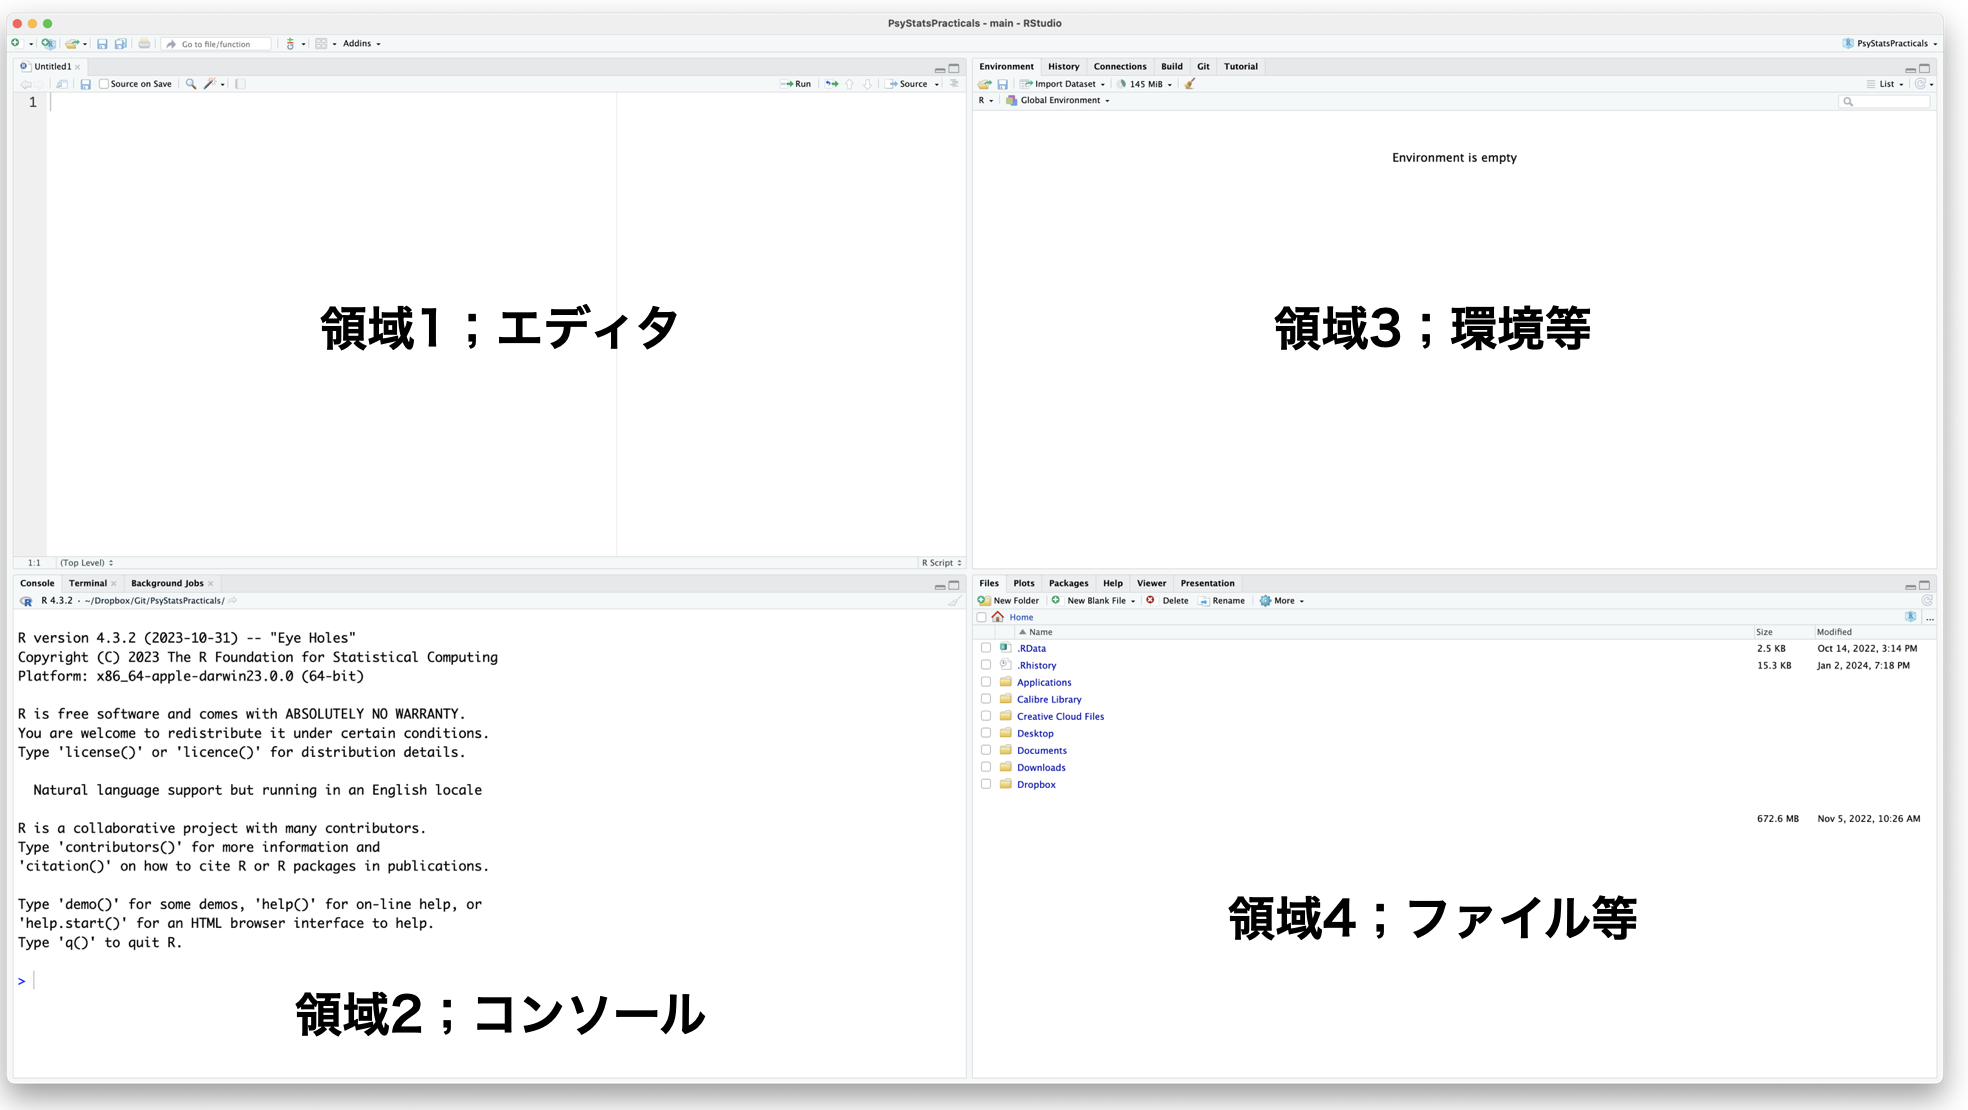
\includegraphics{Figs/01_RStudioStart.png}

}

\caption{RStudioの初期画面}

\end{figure}%

このペインのレイアウトは,メニューのTools \textgreater{} Global
Options\ldots{} \textgreater{} Pane
Layoutから変更することもできる。基本的に4分割であることに変わりはないが,自分が利用しやすい位置にレイアウトを変更するとよい。

\begin{figure}[H]

{\centering 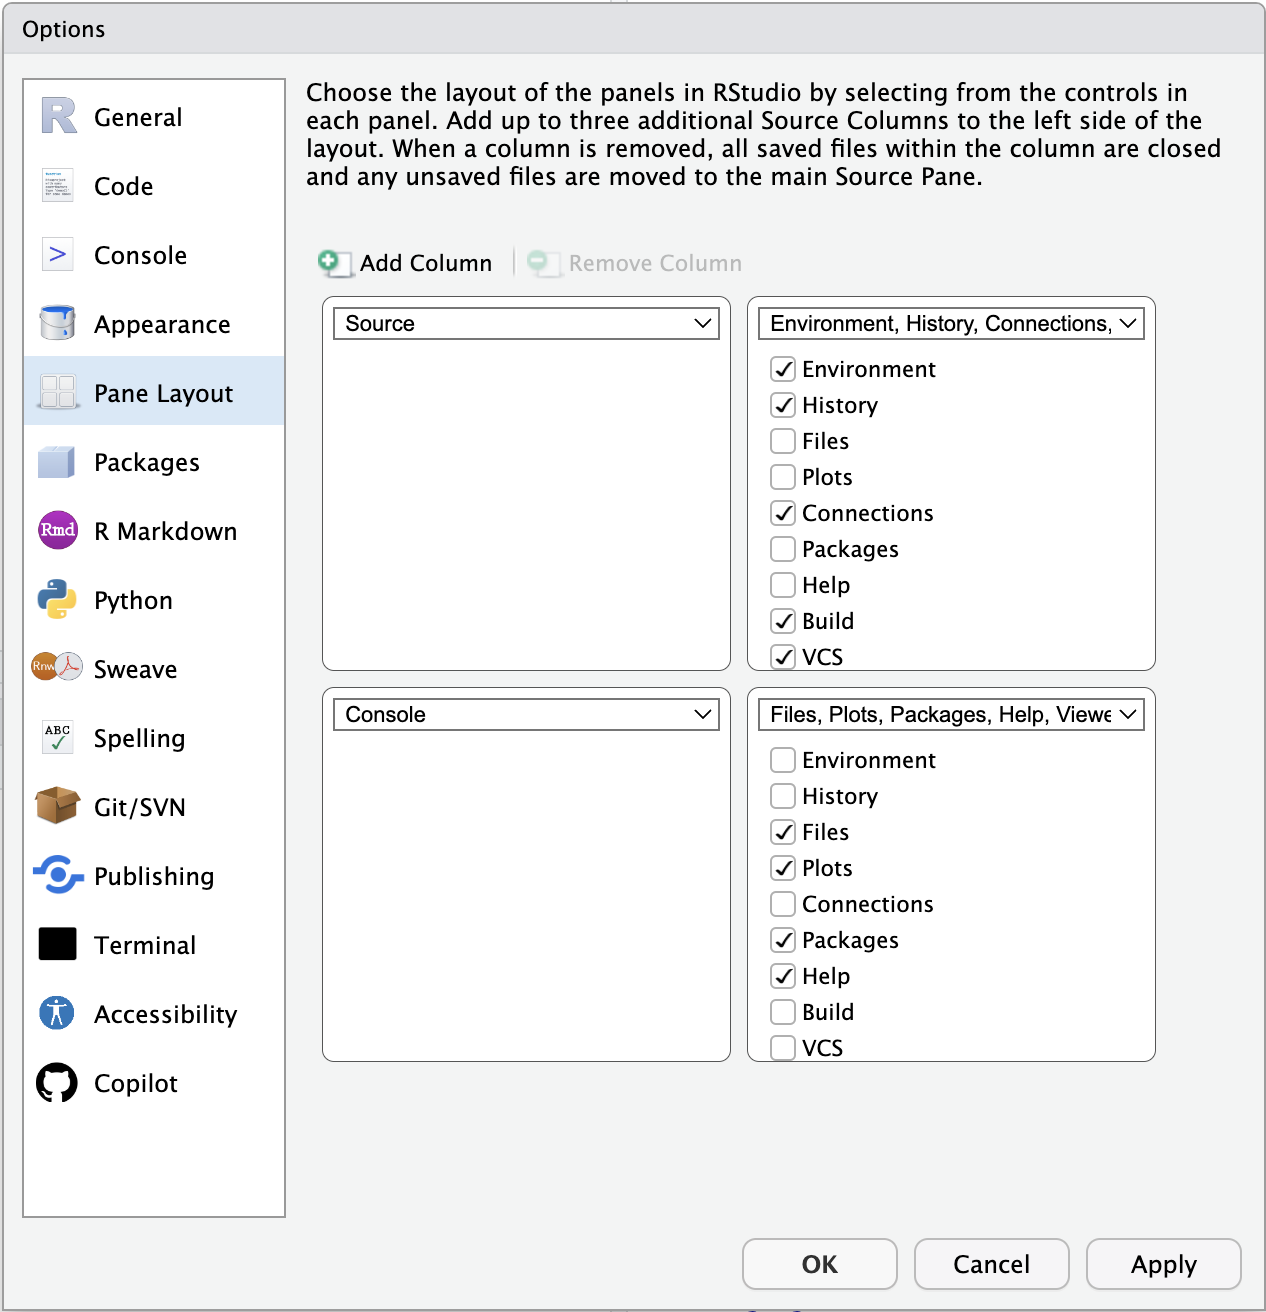
\includegraphics{Figs/01_PaneLayout.png}

}

\caption{レイアウト変更画面。このほかにも背景色などを変えることもできる}

\end{figure}%

以下,各ペイン(領域)が何をするところかを簡単に解説する。

\subsection{領域1;エディタ・ペイン}\label{ux9818ux57df1ux30a8ux30c7ux30a3ux30bfux30daux30a4ux30f3}

エディタ領域。Rのスクリプトはもちろん,レポートの文章など,基本的に入力するときはこのペインに書く。ここで作業するファイルの種類は,File
\textgreater{} New
Fileから見ると明らかなように,R言語だけでなくC言語,Python言語などのスクリプトや,Rmd,md,Qmd,HTMLなどのマークアップ言語,StanやSQLなど特殊な言語などにも対応している。ペインの右下に現在開かれているファイルの種類が表示されているのを確認しておこう。

R言語でスクリプトを書く例で解説しよう。Rは命令を逐次実行していくインタプリタ形式であり,ここに記述されたRコードを,右上のRunボタンでコンソールに送って計算を実行するように使う。一回の命令をコマンド,コマンドが積み重ねられた全体をスクリプト,あるいはプログラムと呼ぶ。複数のコマンドを実行したい場合は,エディタ領域で複数行選択してRunボタンを,スクリプトファイル全体を実行したいときはRunボタンのとなりにあるSourceを押す。CTRL+Enter(Macの場合はコマンド+Enter)でRunボタンのショートカットになる。

\subsection{領域2;コンソール・ペイン}\label{ux9818ux57df2ux30b3ux30f3ux30bdux30fcux30ebux30daux30a4ux30f3}

R単体で利用する場合は,ここのペインだけを利用するようなものである。すなわち,ここに示されているのがR本体というか,Rの計算機能そのものである。ここに「>」の記号が表示されているところをプロンプトといい,プロンプトが表示されているときはRが入力待ちの状態である。

Rは逐次的に計算を行うので,プロンプトのある状態でコマンドを入力すると計算結果が返される。
ここに直接コマンドを書いて行っても良いが,書き間違えたりすることもあるし,コマンドが複数行に渡ることが一般的になってくるので,エディタ領域に清書するつもりで記述していったほうがよい。ごくたまに,一時的に確認したいことがある時だけ,直接コンソールを触るようにすると良い。

なお,コンソールを綺麗にしたいときは右上の箒ボタンをおすとよい。

\subsection{領域3;環境ペイン}\label{ux9818ux57df3ux74b0ux5883ux30daux30a4ux30f3}

基本的にこのペインと次の領域4のペインは複数のタブが含まれる。Pane
Layoutでどちらにどのタブを含めるかを自分好みにカスタマイズすることもできる。ここでは代表的な2つのタブについてのみ言及する。

\textbf{Environment}タブは,Rの実行メモリ内に保管されている変数や関数などが表示されている。「変数や関数など」をまとめて\textbf{オブジェクト}というが,ここで内容や構造をGUIで確認することができる。

\textbf{History}タブは履歴である。これまでコンソールに送られてきたコマンドが順に記録されている。Historyタブからエディタ,コンソールにコマンドを送ることも可能であり,「さっきの命令をもう一度実行したい」といったときに参照すると良い。

\subsection{領域4;ファイルペイン}\label{ux9818ux57df4ux30d5ux30a1ux30a4ux30ebux30daux30a4ux30f3}

ここでも代表的なタブについてのみ解説する。

\textbf{Files}タブはMacでいうFinder,Windowsでいうエクスプローラーのような,ファイル操作画面である。フォルダの作成,ファイルの削除,リネーム,コピーなどの操作が可能である。

\textbf{Plot}タブはRコマンドで描画命令が出された時の結果がここに表示される。RStudioの利点の一つは,このPlotから図をファイルにExportすることが可能であり,その際にファイルサイズやファイル形式を指定できるところにある。

\textbf{Packages}タブは読み込まれているパッケージ,(読み込まれていないが)保管しているパッケージのリストが表示されている。新しくパッケージを導入するときも,ここのinstallボタンから可能であり,保管しているパッケージのアップデートもボタンひとつで可能である。なお,パッケージについては後ほど言及する。

\textbf{Help}タブはRコマンドでヘルプを表示する命令(\texttt{help}関数)が実行された時の結果が表示される領域である。ヘルプを使うことで関数の引数,戻り値,使用例などを参照できる。

\subsection{そのほかのタブ}\label{ux305dux306eux307bux304bux306eux30bfux30d6}

そのほか,表示の有無もオプションになっているようないくつかのタブについて,簡単に解説しておく。

\textbf{Connections}タブはRを外部データベースなどに繋げるときに参照する。大規模データをローカルにすべて取り込むことなく,SQLで必要なテーブルだけ取り出すといった操作をする際は必要になってくるだろう。

\textbf{Git}タブはR,とくにRプロジェクト(後述)のバージョンを管理するときに利用する。Gitとは複数のプログラマによって同時並行的にプログラムを作っていく時の管理システムである。時系列的な差分の記録を得意とするシステムなので,レポートの作成時などに応用すればラボノートの記録としても利用できる。

\textbf{Build}タブはRパッケージやWebサイトを構築するときに利用する。なおこの資料もRStudioを利用して作られており,資料を生成(原稿からHTMLやPDFにする)ときにはこのタブを利用している。

\textbf{Tutorial}タブはチュートリアルツアーを楽しむ時のタブである。

\textbf{Viewer}タブはRStudioで作られたHTMLやPDFなどを見るためのタブである。

\textbf{Presentation}タブはRStudioで作られたプレゼンテーションを見るためのタブである。

\textbf{Terminal}タブはWindows/MacでいうTerminal,Linuxでいう端末についてのタブであり,Rに限らず,コマンドラインを通じてOSに命令するときに使う。

\textbf{Background
Jobs}タブはその名の通りバックグラウンドで作業をさせるときに利用する。Rは基本的にシングルコアで計算が実行されるが,このタブを使ってスクリプトファイルをバックグラウンドで実行することで並列的に作業が可能になる。

\section{Rのパッケージ}\label{rux306eux30d1ux30c3ux30b1ux30fcux30b8}

Rは単体でも線型モデルなどの基本的な分析は可能であるが,より進んだ統計モデルを利用したい場合は専門の\textbf{パッケージ}を導入することになる。パッケージとは関数群のことであり,これもCRANやGithubなどインターネットを介して提供されている。ちなみに提供されているパッケージは,CRANで公開されているものだけで344,607件あり\footnote{2024年01月18日調べ},Github\footnote{Gitはバージョン管理システムであるが,これをインターネット上のサーバ(レポジトリ)で行うものをGithubという。RStudioはGithubとも連携しており,プロジェクトをGithubと紐づけることで簡単にバージョン管理ができる。しかもここで言及しているように,Github上でパッケージを公開することもできるので,最近はCRANの校閲を待たずに公開できるGithubが好まれている側面もある。}で公開されているものなど,CRANを介さないパッケージも少なくない。

パッケージを利用する際は,まずローカルにパッケージファイルをインストールしなければならない。その上で,Rを起動するごとに(セッションごとに),関数\texttt{library}でパッケージを呼び出して利用する。インストールを毎回行う必要はないことに注意。

インストールはRのコマンドでも可能だが,RStudioのPackagesペインを使って導入するのが簡単だろう。以下に,一部の有名かつ有用なパッケージ名とその簡単な説明を挙げる。本講義の中で使うものもあるので,事前に準備しておくことが望ましい。

\begin{itemize}
\tightlist
\item
  \emph{tidyverse}パッケージ\autocite{tidyverse};Rが飛躍的に使いやすくなったのは,このtidyverseパッケージ導入以後のことである。開発者のHadley
  WickhamはR業界で神と崇められており,R業界に与えたインパクトは大きい。このパッケージは「パッケージ群」「パッケージのパッケージ」であり,tidyverseとはtidyな(整然とした)verse(世界)というような意味合いである。このパッケージは統計分析モデルを提供するものではなく,その前のデータの\textbf{前処理}に関する便利な関数を提供する\footnote{実は統計データの解析にかかる時間のほとんどが,解析に適切な形にデータを整形する「前処理」に費やされる。前処理,別名データハンドリングをいかに上手く,素早く,直感的にできるかは,その後の分析にも影響するほど重要な手順であるため,tidyverseパッケージの登場はありがたかった。これを使ったデータハンドリングだけの専門書\autocite{Kinosady2021}が重宝されるほどである。}。このパッケージをインストールすると,関連する依存パッケージが次々取り込まれるので,少々時間がかかる。
\item
  \emph{psych}パッケージ\autocite{psych};名前の通り,心理学統計に関する統計モデルの多くが含まれている。特に特殊な相関係数や,因子分析モデルなどは非常に便利なので,インストールしておいて間違いない。
\item
  \emph{GPArotation}パッケージ\autocite{GPArotation};因子分析における因子軸の回転に使うパッケージ。
\item
  \emph{styler}パッケージ;スタイルを整えてくれるパッケージ。スクリプトの清書に便利。
\item
  \emph{lavaan}パッケージ\autocite{lavaan};潜在変数を含んだモデル(LAtent
  VAriable ANalysis)の分析,要するに構造方程式モデリング(Structural
  Equation Modeling;SEM,共分散構造分析ともいう)を実行するパッケージ。
\item
  \emph{ctv}パッケージ\autocite{CTV}; CRAN Task
  Viewsの略で,膨大に膨れ上がったCRANから必要なパッケージを見つけ出すのは困難であることから,ある程度のジャンルごとに関連しそうなパッケージをまとめて導入してくれるのがこのパッケージ。例えば,このパッケージをインストールした後で,\texttt{install.views("Psychometrics")}とすると,心理統計関係の多くのパッケージを次々導入してくれる。
\item
  \emph{cmdstanr}パッケージ\autocite{cmdstanr};複雑な統計モデルで利用される,確率的プログラミング言語stanをRから使うことができるようになるパッケージ。導入にはこのパッケージの他にもstanやコンパイル環境の準備が必要なので,\href{https://mc-stan.org/cmdstanr/articles/cmdstanr.html}{公式の導入サイト}も参考にしてほしい。
\end{itemize}

\section{RStudioのプロジェクト}\label{rstudioux306eux30d7ux30edux30b8ux30a7ux30afux30c8}

実際にRを使っていく前に,最後の準備としてRStudioにおけるプロジェクトについて解説しておく。

みなさんも,PCをつかって文書を作ったり保管したりするときに,フォルダにまとめて入れておくことがあるだろう。フォルダは例えば「文書」\textgreater「心理学」\textgreater「心理学統計演習」のように階層的に整理することが一般的で,そうしておくことで必要なファイルをすぐに取り出すことができる。

逆に言えば,こうしたフォルダ管理をしておかなければファイルがPCのなかで散乱してしまい,必要な情報を得るために逐一PCの中身を検索しなければならないだろう。

R/RStudioをつかった分析実践の場合も同様で,一回のテーマについて複数のファイル(スクリプトファイル,データファイル,画像ファイル,レポートなど文書ファイル等々)があり,シーンに合わせて(例えば「授業」「卒論」など)フォルダで管理することになる。

さらに,PC環境には作業フォルダ(Working
Directory)\footnote{ここでは,フォルダとディレクトリは同じ意味であると思ってもらって良い。一般に,CUIではディレクトリ,GUIではフォルダという用語が好まれる。語幹directにあるように,ファイルやアクセス先など具体的な指し示す先を強調しているのがディレクトリであり,それにファイル群などまとまった容れもの,という意味を付加したのがフォルダである。フォルダの方が言葉としてわかりやすいし。}という概念がある。たとえばR/RStudioを起動・実行しているときに,Rが「今どこで」実行されているか,どこを管理場所としているか,を表す概念である。例えばこの作業フォルダの中に\texttt{sample.csv}というファイルがあって,それをスクリプト上から読み込みたい,というコマンドを実行するのであれば,そのままファイル名を書けば良い。しかし別の場所にそのファイルが保存されているのなら,作業フォルダから見た相対的な位置を含めて指示してやるか(相対パス),あるいはPC環境全体からみた絶対的な位置を含めて(絶対パス)指示してやる必要がある。相対・絶対パスの違いは,「ここから二つ目の角を右」のように指示するか,住所で指示するかの違いであると考えれば良い。

ともあれ,この作業フォルダがどこに設定されているかは,実行するときに常に気にしていなければならない。ちなみにこの作業フォルダは,RStudioのファイルペイン・Filesタブでひらいているところとは\textbf{限らない}ことに注意してほしい。GUI上でエクスプローラ/Finderで開いたからといって,作業フォルダが自動的に切り替わるようにはなっていない。

そこでRStudioのプロジェクトである。RStudioには「プロジェクト」という概念があり,作業フォルダや環境の設定などをそこで管理することができる。新しくプロジェクトを始めるときはFile\textgreater New
Project,すでに一度プロジェクトを作っているときはFile \textgreater{}
Open
Projectとしてプロジェクトファイル(拡張子が.projのファイル)を開くようにする。そうすると,作業フォルダが当該フォルダに設定される。プロジェクトをGitに連携しておくとバージョン管理などもフォルダ単位で行える。

以後,本講義で外部ファイルを参照する場合,プロジェクトフォルダの中にそのファイルがあるものとして(パスを必要としない形で)論じるので注意されたし。

\section{課題}\label{ux8ab2ux984c}

\begin{itemize}
\tightlist
\item
  Rの最新版をCRANからダウンロードし,自分のPCにインストールしてください。
\item
  RStudioのDesktop版を\href{https://posit.co/download/rstudio-desktop/}{Posit社のサイト}からダウンロードし,自分のPCにインストールしてください。
\item
  RStidoを起動し,ペインレイアウトをデフォルトではない状態に並べ直してみてください。ソースペインを3列にするのも良いでしょう。
\item
  コンソールペインに書かれている文字を全て消去してみてください。
\item
  ファイルペインにあるFilesタブをつかって,色々なフォルダを開けてみたり,不要なファイルを削除したり,ファイル名を変更したりしてみてください。
\item
  ファイルペインにあるFilesタブを開き,\texttt{More}のところから\texttt{Go\ To\ Working\ Directory}を選択・実行してください。何か起こったでしょうか。
\item
  この授業のために,新しいプロジェクトを作成してください。プロジェクトは新しいフォルダでも,既存のフォルダでも構いません。
\item
  プロジェクトが開いた状態のとき,RStudioのウィンドウ・タブのどこかに「プロジェクト名」が表示されているはずです。確認してください。
\item
  またファイルペインのFilesタブから,色々なファイル操作をした上で,改めて\texttt{Go\ To\ Working\ Directory}をしてください。プロジェクトフォルダの中に戻ってこれたら成功です。
\item
  新しいRスクリプトファイルを開き,空白のままで結構ですからファイル名をつけて保存してください。
\item
  RStudioを終了あるいは最小化させ,OSのエクスプローラ/Finderから,プロジェクトフォルダに移動してください。先ほど作ったファイルが保存されていることを確認してください。
\item
  プロジェクトフォルダには,プロジェクト名+\texttt{.proj}というファイルが存在するはずです。これを開いて,RStudioのプロジェクトを開いてください。
\item
  RStudioのFile \textgreater{} Close
  Projectからプロジェクトを閉じてください。画面の細部でどこが変わったか,確認してください。
\item
  RStudioを終了し,再びRStudioを起動してください。起動の方法はプロジェクトファイルからでも,アプリケーションの起動でも構いません。起動後に,プロジェクトを開いてください(あるいはプロジェクトが開かれていることを確認してください。)。
\end{itemize}

\section{References}\label{references}

\printbibliography[heading=none]

\bookmarksetup{startatroot}

\chapter{Rの基礎}\label{rux306eux57faux790e}

ここから実際にR/RStudioをつかった演習に入る。前回すでに言及したように,この講義ようのプロジェクトを準備し,RStudioはプロジェクトが開かれた状態であることを前提に話を進める。

\section{Rで計算}\label{rux3067ux8a08ux7b97}

まずはRを使った計算である。Rスクリプトファイルを開き,最初の行に次の4行を入力してみよう。
各行を実行(Runボタン,あるいはctrl+enter)し,コンソールの結果を確認しよう。

\begin{Shaded}
\begin{Highlighting}[]
\DecValTok{1} \SpecialCharTok{+} \DecValTok{2}
\end{Highlighting}
\end{Shaded}

\begin{verbatim}
[1] 3
\end{verbatim}

\begin{Shaded}
\begin{Highlighting}[]
\DecValTok{2} \SpecialCharTok{{-}} \DecValTok{3}
\end{Highlighting}
\end{Shaded}

\begin{verbatim}
[1] -1
\end{verbatim}

\begin{Shaded}
\begin{Highlighting}[]
\DecValTok{3} \SpecialCharTok{*} \DecValTok{4}
\end{Highlighting}
\end{Shaded}

\begin{verbatim}
[1] 12
\end{verbatim}

\begin{Shaded}
\begin{Highlighting}[]
\DecValTok{6} \SpecialCharTok{/} \DecValTok{3}
\end{Highlighting}
\end{Shaded}

\begin{verbatim}
[1] 2
\end{verbatim}

それぞれ加減乗除の計算結果が正しく出ていることを確認してほしい。なお,出力のところに\texttt{{[}1{]}}とあるのは,Rがベクトルを演算の基本としているからで,回答ベクトルの第1要素を返していることを意味する。

四則演算の他に,次のような演算も可能である。

\begin{Shaded}
\begin{Highlighting}[]
\CommentTok{\# 整数の割り算}
\DecValTok{8} \SpecialCharTok{\%/\%} \DecValTok{3}
\end{Highlighting}
\end{Shaded}

\begin{verbatim}
[1] 2
\end{verbatim}

\begin{Shaded}
\begin{Highlighting}[]
\CommentTok{\# 余り}
\DecValTok{7} \SpecialCharTok{\%\%} \DecValTok{3}
\end{Highlighting}
\end{Shaded}

\begin{verbatim}
[1] 1
\end{verbatim}

\begin{Shaded}
\begin{Highlighting}[]
\CommentTok{\# 冪乗}
\DecValTok{2}\SpecialCharTok{\^{}}\DecValTok{3}
\end{Highlighting}
\end{Shaded}

\begin{verbatim}
[1] 8
\end{verbatim}

ここで,\texttt{\#}から始まる行は\textbf{コメントアウト}されたものとして,実際にコンソールに送られても計算されないことに注意しよう。スクリプトが単純なものである場合はコメントをつける必要はないが,複雑な計算になったり,他者と共有するときは「今どのような演算をしているか」を逐一解説するようにすると便利である。

実践上のテクニックとして,複数行を一括でコメントアウトしたり,アンコメント(コメントアウトを解除する)したりすることがある。スクリプトを複数行選択した上で,Codeメニューから\texttt{Comment/Uncomment\ Lines}を押すとコメント/アンコメントを切り替えられるので試してみよう。また,ショートカットキーも確認し,キーからコメント/アンコメントができるように慣れておくと良い(Ctrl+↑+C/Cmd+↑+C)。

One more
tips.コメントではなく,大きな段落的な区切り(セクション区切り)が欲しいこともあるかもしれない。Codeメニューの一番上に「Insert
Section」があるのでこれを選んでみよう。ショートカットキーから入力しても良い(Ctrl+↑+R/Cmd+↑+R)。セクション名を入力するボックスに適当な命名をすると,スクリプトにセクションが挿入される。次に示すのがセクションの例である。

\begin{Shaded}
\begin{Highlighting}[]
\CommentTok{\# 計算 {-}{-}{-}{-}{-}{-}{-}{-}{-}{-}{-}{-}{-}{-}{-}{-}{-}{-}{-}{-}{-}{-}{-}{-}{-}{-}{-}{-}{-}{-}{-}{-}{-}{-}{-}{-}{-}{-}{-}{-}{-}{-}{-}{-}{-}{-}{-}{-}{-}{-}{-}{-}{-}{-}{-}{-}{-}{-}{-}{-}{-}{-}}
\end{Highlighting}
\end{Shaded}

これはもちろん実行に影響を与えないが,ソースが長くなった場合はこのセクション単位で移動したり(スクリプトペインの左下),アウトラインを確認したり(スクリプトペインの右上にある横三本線)できるので,活用して欲しい。

\section{オブジェクト}\label{ux30aaux30d6ux30b8ux30a7ux30afux30c8}

Rでは変数,関数などあらゆるものを\textbf{オブジェクト}としてあつかう。オブジェクトには任意の名前をつけることができる(数字から始まる名前は不可)。
オブジェクトを作り,そこにある値を\textbf{代入}する例は次の通りである。

\begin{Shaded}
\begin{Highlighting}[]
\NormalTok{a }\OtherTok{\textless{}{-}} \DecValTok{1}
\NormalTok{b }\OtherTok{\textless{}{-}} \DecValTok{2}
\NormalTok{A }\OtherTok{\textless{}{-}} \DecValTok{3}
\NormalTok{a }\SpecialCharTok{+}\NormalTok{ b }\CommentTok{\# 1 + 2におなじ}
\end{Highlighting}
\end{Shaded}

\begin{verbatim}
[1] 3
\end{verbatim}

\begin{Shaded}
\begin{Highlighting}[]
\NormalTok{A }\SpecialCharTok{+}\NormalTok{ b }\CommentTok{\# 3 + 2におなじ}
\end{Highlighting}
\end{Shaded}

\begin{verbatim}
[1] 5
\end{verbatim}

ここでは数字をオブジェクトに保管し,オブジェクトを使って計算をしている。大文字と小文字が区別されてるため,計算結果が異なることに注意。

代入に使った記号\texttt{\textless{}-}は「小なり」と「ハイフン」であるが,左矢印のイメージである。次のように,\texttt{=}や\texttt{-\textgreater{}}を使うこともできる。

\begin{Shaded}
\begin{Highlighting}[]
\NormalTok{B }\OtherTok{=} \DecValTok{5}
\DecValTok{7} \OtherTok{{-}\textgreater{}}\NormalTok{ A}
\end{Highlighting}
\end{Shaded}

ここで,二行目に\texttt{7\ -\textgreater{}\ A}を行った。先ほど\texttt{A\ \textless{}-\ 3}としたが,その後に\texttt{A}には7を代入し直したので,値は上書きされる。

\begin{Shaded}
\begin{Highlighting}[]
\NormalTok{A }\SpecialCharTok{+}\NormalTok{ b }\CommentTok{\# 7 + 2におなじ}
\end{Highlighting}
\end{Shaded}

\begin{verbatim}
[1] 9
\end{verbatim}

このように,オブジェクトに代入を重ねると,警告などなしに上書きされることに注意して欲しい。似たようなオブジェクト名を使い回していると,本来意図していたものと違う値・状態を保管していることになりかねないからである。

ちなみに,オブジェクトの中身を確認するためには,そのままオブジェクト名を入力すれば良い。より丁寧には,\texttt{print}関数を使う。

\begin{Shaded}
\begin{Highlighting}[]
\NormalTok{a}
\end{Highlighting}
\end{Shaded}

\begin{verbatim}
[1] 1
\end{verbatim}

\begin{Shaded}
\begin{Highlighting}[]
\FunctionTok{print}\NormalTok{(A)}
\end{Highlighting}
\end{Shaded}

\begin{verbatim}
[1] 7
\end{verbatim}

あるいは,RStudioのEnvironmentタブをみると,現在Rが保持しているオブジェクトが確認でき,単一の値の場合はValueセクションにオブジェクト名と値を見ることができる。

注意点として,オブジェクト名として,次の名前は使うことができない。>
break, else, for, if, in, next, function, repeat, return, while, TRUE,
FALSE.

これらはRで特別な意味を持つ\textbf{予約語}と呼ぶ。特に\texttt{TRUE}と\texttt{FALSE}は真・偽を表すもので,大文字の\texttt{T},\texttt{F}でも代用できるため,この一文字だけをオブジェクト名にするのは避けた方が良い。

\section{関数}\label{ux95a2ux6570}

関数は一般に\(y=f(x)\)と表されるが,要するに\(x\)を与えると\(y\)に形が変わる作用のことを指す。
プログラミング言語では一般に,\(x\)を\textbf{引数(ひきすう,argument)},\(y\)を\textbf{戻り値(もどりち,value)}という。以下,関数の使用例を挙げる。

\begin{Shaded}
\begin{Highlighting}[]
\FunctionTok{sqrt}\NormalTok{(}\DecValTok{16}\NormalTok{)}
\end{Highlighting}
\end{Shaded}

\begin{verbatim}
[1] 4
\end{verbatim}

\begin{Shaded}
\begin{Highlighting}[]
\FunctionTok{help}\NormalTok{(}\StringTok{"sqrt"}\NormalTok{)}
\end{Highlighting}
\end{Shaded}

最初の例は平方根square
rootを取る関数\texttt{sqrt}であり,引数として数字を与えるとその平方根が返される。第二の例は関数の説明を表示させる関数\texttt{help}であり,これを実行するとヘルプペインに関数の説明が表示される。

\section{変数の種類}\label{ux5909ux6570ux306eux7a2eux985e}

先ほどの\texttt{help}関数に与えた引数\texttt{"sqrt"}は文字列である。文字列であることを明示するためにダブルクォーテーション(\texttt{"})で囲っている(シングルクォーテーションで囲っても良い)。このように,Rが扱う変数は数字だけではない。変数の種類は数値型(numeric),文字型(character),論理値(logical)の3種類がある。

\begin{Shaded}
\begin{Highlighting}[]
\NormalTok{obj1 }\OtherTok{\textless{}{-}} \FloatTok{1.5}
\NormalTok{obj2 }\OtherTok{\textless{}{-}} \StringTok{"Hello"}
\NormalTok{obj3 }\OtherTok{\textless{}{-}} \ConstantTok{TRUE}
\end{Highlighting}
\end{Shaded}

数値型は整数(integer),実数(double)を含み\footnote{実数はreal
  numberじゃないのか,という指摘もあろうかとおもう。ここでは電子計算機上の数値の分類である,倍精度浮動小数点数(double-precision
  floating-point
  number)の意味である。倍精度とは単精度の倍を意味しており,単精度は32ビットを,倍精度は64ビットを単位として一つの数字を表す仕組みのことである。},そのほか,複素数型(complex),欠損値を表す\texttt{NA},非数値を表す\texttt{NaN}(Not
a Number),無限大を表す\texttt{Inf}などがある。

文字型はすでに説明した通りで,対になるクォーテーションが必要であることに注意してほしい。終わりを表すクォーテーションがなければ,Rは続く数字や文字も含めた「語」として処理する。この場合,enterキーを押しても文字入力が閉じられていないため,コンソールには「+」の表示が出る(この記号は前の行から入力が続いており,プロンプト状態ではないことを表している)。

また,文字型は当然のことながら四則演算の対象にならない。ただし,論理型の\texttt{TRUE/FALSE}はそれぞれ1,0に対応しているため,計算結果が表示される。次のコードを実行してこのことを確認しよう。

\begin{Shaded}
\begin{Highlighting}[]
\NormalTok{obj1 }\SpecialCharTok{+}\NormalTok{ obj2}
\NormalTok{obj1 }\SpecialCharTok{+}\NormalTok{ obj3}
\end{Highlighting}
\end{Shaded}

\section{オブジェクトの型}\label{ux30aaux30d6ux30b8ux30a7ux30afux30c8ux306eux578b}

ここまでみてきたように,数値や文字など(まとめて\textbf{リテラル}という)にも種類があるが,これをストックしておくものは全て\textbf{オブジェクト}である。オブジェクトとは変数のこと,と理解しても良いが,関数もオブジェクトに含まれる。

\subsection{ベクトル}\label{ux30d9ux30afux30c8ux30eb}

Rのオブジェクトは単一の値しか持たないものではない。むしろ,複数の要素をセットで持つことができるのが特徴である。次に示すのは,\textbf{ベクトル}オブジェクトの例である。

\begin{Shaded}
\begin{Highlighting}[]
\NormalTok{vec1 }\OtherTok{\textless{}{-}} \FunctionTok{c}\NormalTok{(}\DecValTok{2}\NormalTok{, }\DecValTok{4}\NormalTok{, }\DecValTok{5}\NormalTok{)}
\NormalTok{vec2 }\OtherTok{\textless{}{-}} \DecValTok{1}\SpecialCharTok{:}\DecValTok{3}
\NormalTok{vec3 }\OtherTok{\textless{}{-}} \DecValTok{7}\SpecialCharTok{:}\DecValTok{5}
\NormalTok{vec4 }\OtherTok{\textless{}{-}} \FunctionTok{seq}\NormalTok{(}\AttributeTok{from =} \DecValTok{1}\NormalTok{, }\AttributeTok{to =} \DecValTok{7}\NormalTok{, }\AttributeTok{by =} \DecValTok{2}\NormalTok{)}
\NormalTok{vec5 }\OtherTok{\textless{}{-}} \FunctionTok{c}\NormalTok{(vec2, vec3)}
\end{Highlighting}
\end{Shaded}

それぞれのオブジェクトの中身を確認しよう。
最初の\texttt{c()}は結合combine関数である。また,コロン(\texttt{:})は連続する数値を与える。
\texttt{seq}関数は複数の引数を取るが,初期値,終了値,その間隔を指定した連続的なベクトルを生成する関数である。

ベクトルの計算は要素ごとに行われる。次のコードを実行し,どのように振る舞うか確認しよう。

\begin{Shaded}
\begin{Highlighting}[]
\NormalTok{vec1 }\SpecialCharTok{+}\NormalTok{ vec2}
\end{Highlighting}
\end{Shaded}

\begin{verbatim}
[1] 3 6 8
\end{verbatim}

\begin{Shaded}
\begin{Highlighting}[]
\NormalTok{vec3 }\SpecialCharTok{*} \DecValTok{2}
\end{Highlighting}
\end{Shaded}

\begin{verbatim}
[1] 14 12 10
\end{verbatim}

\begin{Shaded}
\begin{Highlighting}[]
\NormalTok{vec1 }\SpecialCharTok{+}\NormalTok{ vec5}
\end{Highlighting}
\end{Shaded}

\begin{verbatim}
[1]  3  6  8  9 10 10
\end{verbatim}

最後の計算でエラーが出なかったことに注目しよう。たとえば\texttt{vec1\ +\ vec4}はエラーになるが,ここでは計算結果が示されている(=エラーにはなっていない)。数学的には,長さの違うベクトルは計算が定義されていないのだが,\texttt{vec1}の長さは3,\texttt{vec5}の長さは6であった。\textbf{Rはベクトルを再利用する}ので,長いベクトルが短いベクトルの定数倍になるときは反復して利用される。すなわち,ここでは
\[ (2,4,5,2,4,5) + (1,2,3,7,6,5) = (3,6,8,9,10,10)\]
の計算がなされた。このRの仕様については,意図せぬ挙動にならぬよう注意しよう。

ベクトルの要素にアクセスするときは大括弧(\texttt{{[}\ {]}})を利用する。
特に第二・第三行目のコードの使い方を確認しておこう。大括弧の中は,要素番号でも良いし,真/偽の判断でも良いのである。この真偽判断による指定の方法は,条件節(\texttt{if}文)をつかって要素を指定できるため,有用である。

\begin{Shaded}
\begin{Highlighting}[]
\NormalTok{vec1[}\DecValTok{2}\NormalTok{]}
\end{Highlighting}
\end{Shaded}

\begin{verbatim}
[1] 4
\end{verbatim}

\begin{Shaded}
\begin{Highlighting}[]
\NormalTok{vec2[}\FunctionTok{c}\NormalTok{(}\DecValTok{1}\NormalTok{, }\DecValTok{3}\NormalTok{)]}
\end{Highlighting}
\end{Shaded}

\begin{verbatim}
[1] 1 3
\end{verbatim}

\begin{Shaded}
\begin{Highlighting}[]
\NormalTok{vec2[}\FunctionTok{c}\NormalTok{(}\ConstantTok{TRUE}\NormalTok{, }\ConstantTok{FALSE}\NormalTok{, }\ConstantTok{TRUE}\NormalTok{)]}
\end{Highlighting}
\end{Shaded}

\begin{verbatim}
[1] 1 3
\end{verbatim}

ここまで,ベクトルの要素は数値で説明してきたが,文字列などもベクトルとして利用できる。

\begin{Shaded}
\begin{Highlighting}[]
\NormalTok{words1 }\OtherTok{\textless{}{-}} \FunctionTok{c}\NormalTok{(}\StringTok{"Hello!"}\NormalTok{, }\StringTok{"Mr."}\NormalTok{, }\StringTok{"Monkey"}\NormalTok{, }\StringTok{"Magic"}\NormalTok{, }\StringTok{"Orchestra"}\NormalTok{)}
\NormalTok{words1[}\DecValTok{3}\NormalTok{]}
\end{Highlighting}
\end{Shaded}

\begin{verbatim}
[1] "Monkey"
\end{verbatim}

\begin{Shaded}
\begin{Highlighting}[]
\NormalTok{words2 }\OtherTok{\textless{}{-}}\NormalTok{ LETTERS[}\DecValTok{1}\SpecialCharTok{:}\DecValTok{10}\NormalTok{]}
\NormalTok{words2[}\DecValTok{8}\NormalTok{]}
\end{Highlighting}
\end{Shaded}

\begin{verbatim}
[1] "H"
\end{verbatim}

ここで\texttt{LETTERS}はアルファベット26文字が含まれている予約語ベクトルである。

ベクトルを引数に取る関数も多い。たとえば記述統計量である,平均,分散,標準偏差,合計などは,次のようにして計算する。

\begin{Shaded}
\begin{Highlighting}[]
\NormalTok{dat }\OtherTok{\textless{}{-}} \FunctionTok{c}\NormalTok{(}\DecValTok{12}\NormalTok{,}\DecValTok{18}\NormalTok{,}\DecValTok{23}\NormalTok{,}\DecValTok{35}\NormalTok{,}\DecValTok{22}\NormalTok{)}
\FunctionTok{mean}\NormalTok{(dat) }\CommentTok{\# 平均}
\end{Highlighting}
\end{Shaded}

\begin{verbatim}
[1] 22
\end{verbatim}

\begin{Shaded}
\begin{Highlighting}[]
\FunctionTok{var}\NormalTok{(dat)  }\CommentTok{\# 分散}
\end{Highlighting}
\end{Shaded}

\begin{verbatim}
[1] 71.5
\end{verbatim}

\begin{Shaded}
\begin{Highlighting}[]
\FunctionTok{sd}\NormalTok{(dat)   }\CommentTok{\# 標準偏差}
\end{Highlighting}
\end{Shaded}

\begin{verbatim}
[1] 8.455767
\end{verbatim}

\begin{Shaded}
\begin{Highlighting}[]
\FunctionTok{sum}\NormalTok{(dat)  }\CommentTok{\# 合計}
\end{Highlighting}
\end{Shaded}

\begin{verbatim}
[1] 110
\end{verbatim}

他にも最大値\texttt{max}や最小値\texttt{min},中央値\texttt{median}などの関数が利用可能である。

\subsection{行列}\label{ux884cux5217}

数学では線形代数でベクトルを扱うが,同時にベクトルが複数並んだ二次元の行列も扱うだろう。
Rでも行列のように配置したオブジェクトを利用できる。

次のコードで作られる行列\(A\),\(B\)がどのようなものか確認しよう。

\begin{Shaded}
\begin{Highlighting}[]
\NormalTok{A }\OtherTok{\textless{}{-}} \FunctionTok{matrix}\NormalTok{(}\DecValTok{1}\SpecialCharTok{:}\DecValTok{6}\NormalTok{, }\AttributeTok{ncol =} \DecValTok{2}\NormalTok{)}
\NormalTok{B }\OtherTok{\textless{}{-}} \FunctionTok{matrix}\NormalTok{(}\DecValTok{1}\SpecialCharTok{:}\DecValTok{6}\NormalTok{, }\AttributeTok{ncol =} \DecValTok{2}\NormalTok{, }\AttributeTok{byrow =}\NormalTok{ T)}
\end{Highlighting}
\end{Shaded}

行列を作る関数\texttt{matrix}は,引数として要素,列数(\texttt{ncol}),行数(\texttt{nrow}),要素配列を行ごとにするかどうかの指定(\texttt{byrow})をとる。ここでは要素を\texttt{1:6}としており,1から6までの連続する整数をあたえている。\texttt{ncol}で2列であることを明示しているので,\texttt{nrow}で行数を指定してやる必要はない。\texttt{byrow}の有無でどのように数字が変わっているかは表示させれば一目瞭然であろう。

与える要素が行数\(\times\)列数に一致しておらず,ベクトルの再利用も不可能な場合はエラーが返ってくる。

また,ベクトルの要素指定のように,行列も大括弧を使って要素を指定することができる。行,列の順に指定し,行だけ,列だけの指定も可能である。

\begin{Shaded}
\begin{Highlighting}[]
\NormalTok{A[}\DecValTok{2}\NormalTok{, }\DecValTok{2}\NormalTok{]}
\end{Highlighting}
\end{Shaded}

\begin{verbatim}
[1] 5
\end{verbatim}

\begin{Shaded}
\begin{Highlighting}[]
\NormalTok{A[}\DecValTok{1}\NormalTok{, ]}
\end{Highlighting}
\end{Shaded}

\begin{verbatim}
[1] 1 4
\end{verbatim}

\begin{Shaded}
\begin{Highlighting}[]
\NormalTok{A[, }\DecValTok{2}\NormalTok{]}
\end{Highlighting}
\end{Shaded}

\begin{verbatim}
[1] 4 5 6
\end{verbatim}

\subsection{リスト型}\label{ux30eaux30b9ux30c8ux578b}

行列はサイズの等しいベクトルのセットであるが,サイズの異なる要素をまとめて一つのオブジェクトとして保管しておきたいときはリスト型をつかう。

\begin{Shaded}
\begin{Highlighting}[]
\NormalTok{Obj1 }\OtherTok{\textless{}{-}} \FunctionTok{list}\NormalTok{(}\DecValTok{1}\SpecialCharTok{:}\DecValTok{4}\NormalTok{, }\FunctionTok{matrix}\NormalTok{(}\DecValTok{1}\SpecialCharTok{:}\DecValTok{6}\NormalTok{, }\AttributeTok{ncol =} \DecValTok{2}\NormalTok{), }\DecValTok{3}\NormalTok{)}
\end{Highlighting}
\end{Shaded}

このオブジェクトの第一要素(\texttt{{[}{[}1{]}{]}})はベクトル,第二要素は行列,第三要素は要素1つのベクトル(スカラー)である。オブジェクトの要素の要素(ex.第二要素の行列の2行3列目の要素)にどのようにアクセスすれば良いか,考えてみよう。

このリストは要素へのアクセスの際に\texttt{{[}{[}1{]}{]}}など数字が必要だが,要素に名前をつけることで利便性が増す。

\begin{Shaded}
\begin{Highlighting}[]
\NormalTok{Obj2 }\OtherTok{\textless{}{-}} \FunctionTok{list}\NormalTok{(}
  \AttributeTok{vec1 =} \DecValTok{1}\SpecialCharTok{:}\DecValTok{5}\NormalTok{,}
  \AttributeTok{mat1 =} \FunctionTok{matrix}\NormalTok{(}\DecValTok{1}\SpecialCharTok{:}\DecValTok{10}\NormalTok{, }\AttributeTok{nrow =} \DecValTok{5}\NormalTok{),}
  \AttributeTok{char1 =} \StringTok{"YMO"}
\NormalTok{)}
\end{Highlighting}
\end{Shaded}

この名前付きリストの要素にアクセスするときは,\texttt{\$}記号を用いることができる。

\begin{Shaded}
\begin{Highlighting}[]
\NormalTok{Obj2}\SpecialCharTok{$}\NormalTok{vec1}
\end{Highlighting}
\end{Shaded}

\begin{verbatim}
[1] 1 2 3 4 5
\end{verbatim}

これを踏まえて,名前付きリストの要素の要素にアクセスするにはどうすれば良いか,考えてみよう。

リスト型はこのように,要素のサイズ・長さを問わないため,いろいろなものを保管しておくことができる。統計関数の結果はリスト型で得られることが多く,そのような場合,リストの要素も長くなりがちである。リストがどのような構造を持っているかを見るために,\texttt{str}関数が利用できる。

\begin{Shaded}
\begin{Highlighting}[]
\FunctionTok{str}\NormalTok{(Obj2)}
\end{Highlighting}
\end{Shaded}

\begin{verbatim}
List of 3
 $ vec1 : int [1:5] 1 2 3 4 5
 $ mat1 : int [1:5, 1:2] 1 2 3 4 5 6 7 8 9 10
 $ char1: chr "YMO"
\end{verbatim}

\texttt{str}関数の返す結果と同じものが,RStudioのEnvironmentタブからオブジェクトを見ることでも得られる。
また,リストの要素としてリストを持つ,すなわち階層的になることもある。そのような場合,必要としている要素にどのようにアクセスすれば良いか,確認しておこう。

\begin{Shaded}
\begin{Highlighting}[]
\NormalTok{Obj3 }\OtherTok{\textless{}{-}} \FunctionTok{list}\NormalTok{(Obj1,}\AttributeTok{Second =}\NormalTok{Obj2)}
\FunctionTok{str}\NormalTok{(Obj3)}
\end{Highlighting}
\end{Shaded}

\begin{verbatim}
List of 2
 $       :List of 3
  ..$ : int [1:4] 1 2 3 4
  ..$ : int [1:3, 1:2] 1 2 3 4 5 6
  ..$ : num 3
 $ Second:List of 3
  ..$ vec1 : int [1:5] 1 2 3 4 5
  ..$ mat1 : int [1:5, 1:2] 1 2 3 4 5 6 7 8 9 10
  ..$ char1: chr "YMO"
\end{verbatim}

\subsection{データフレーム型}\label{ux30c7ux30fcux30bfux30d5ux30ecux30fcux30e0ux578b}

リスト型は要素のサイズを問わないことはすでに述べた。しかしデータ解析を行うときは得てして,2次元スプレッドシートのような形式である。すなわち一行に1オブザベーション,各列は変数を表すといった具合である。このように矩形かつ,列に変数名を持たせることができる特殊なリスト型を\textbf{データフレーム型}という。以下はそのようなオブジェクトの例である。

\begin{Shaded}
\begin{Highlighting}[]
\NormalTok{df }\OtherTok{\textless{}{-}} \FunctionTok{data.frame}\NormalTok{(}
  \AttributeTok{name =} \FunctionTok{c}\NormalTok{(}\StringTok{"Ishino"}\NormalTok{, }\StringTok{"Pierre"}\NormalTok{, }\StringTok{"Marin"}\NormalTok{),}
  \AttributeTok{origin =} \FunctionTok{c}\NormalTok{(}\StringTok{"Shizuoka"}\NormalTok{,}\StringTok{"Shizuoka"}\NormalTok{,}\StringTok{"Hokkaido"}\NormalTok{),}
  \AttributeTok{height =} \FunctionTok{c}\NormalTok{(}\DecValTok{170}\NormalTok{, }\DecValTok{180}\NormalTok{, }\DecValTok{160}\NormalTok{),}
  \AttributeTok{salary =} \FunctionTok{c}\NormalTok{(}\DecValTok{1000}\NormalTok{, }\DecValTok{20}\NormalTok{, }\DecValTok{800}\NormalTok{)}
\NormalTok{)}
\CommentTok{\# 内容を表示させる}
\NormalTok{df}
\end{Highlighting}
\end{Shaded}

\begin{verbatim}
    name   origin height salary
1 Ishino Shizuoka    170   1000
2 Pierre Shizuoka    180     20
3  Marin Hokkaido    160    800
\end{verbatim}

\begin{Shaded}
\begin{Highlighting}[]
\CommentTok{\# 構造を確認する}
\FunctionTok{str}\NormalTok{(df)}
\end{Highlighting}
\end{Shaded}

\begin{verbatim}
'data.frame':   3 obs. of  4 variables:
 $ name  : chr  "Ishino" "Pierre" "Marin"
 $ origin: chr  "Shizuoka" "Shizuoka" "Hokkaido"
 $ height: num  170 180 160
 $ salary: num  1000 20 800
\end{verbatim}

ところで,心理統計の初歩としてStevensの尺度水準\autocite{stevens1946}について学んだことと思う。そこでは数値が,その値に許される演算のレベルをもとに,名義,順序,間隔,比率尺度水準という4つの段階に分類される。間隔・比率尺度水準の数値は数学的な計算を施しても良いが,順序尺度水準や名義尺度水準の数字はそのような計算が許されない(ex.2番目に好きな人と3番目に好きな人が一緒になっても,1番好きな人に敵わない。)

Rには,こうした尺度水準に対応した数値型がある。間隔・比率尺度水準は計算可能なので\texttt{numeric}型でよいが,名義尺度水準は\texttt{factor}型(要因型,因子型とも呼ばれる),順序尺度水準は\texttt{ordered.factor}型と呼ばれるものである。

factor型の変数の例を挙げる。すでに文字型として入っているものをfactor型として扱うよう変換するためには,\texttt{as.factor}関数が利用できる。

\begin{Shaded}
\begin{Highlighting}[]
\NormalTok{df}\SpecialCharTok{$}\NormalTok{origin }\OtherTok{\textless{}{-}} \FunctionTok{as.factor}\NormalTok{(df}\SpecialCharTok{$}\NormalTok{origin)}
\NormalTok{df}\SpecialCharTok{$}\NormalTok{origin}
\end{Highlighting}
\end{Shaded}

\begin{verbatim}
[1] Shizuoka Shizuoka Hokkaido
Levels: Hokkaido Shizuoka
\end{verbatim}

要素を表示させて見ると明らかなように,値としては\texttt{Shizuoka},\texttt{Shizuoka},\texttt{Hokkaido}の3つあるが,レベル(水準)は\texttt{Shizuoka},\texttt{Hokkaido}の2つである。このようにfactor型にしておくと,カテゴリとして使えて便利である。

次に示すのは順序つきfactor型変数の例である。

\begin{Shaded}
\begin{Highlighting}[]
\CommentTok{\# 順序付き要因型の例}
\NormalTok{ratings }\OtherTok{\textless{}{-}} \FunctionTok{factor}\NormalTok{(}\FunctionTok{c}\NormalTok{(}\StringTok{"低い"}\NormalTok{, }\StringTok{"高い"}\NormalTok{, }\StringTok{"中程度"}\NormalTok{, }\StringTok{"高い"}\NormalTok{, }\StringTok{"低い"}\NormalTok{), }
                  \AttributeTok{levels =} \FunctionTok{c}\NormalTok{(}\StringTok{"低い"}\NormalTok{, }\StringTok{"中程度"}\NormalTok{, }\StringTok{"高い"}\NormalTok{), }
                  \AttributeTok{ordered =} \ConstantTok{TRUE}\NormalTok{)}
\CommentTok{\# ratingsの内容と型を確認}
\FunctionTok{print}\NormalTok{(ratings)}
\end{Highlighting}
\end{Shaded}

\begin{verbatim}
[1] 低い   高い   中程度 高い   低い  
Levels: 低い < 中程度 < 高い
\end{verbatim}

集計の際などはfactor型と違わないため,使用例は少ないかもしれない。しかしRは統計モデルを適用する時に,尺度水準に対応した振る舞いをするものがあるので,データの尺度水準を丁寧に設定しておくのも良いだろう。

データフレームの要素へのアクセスは,基本的に変数名を介してのものになるだろう。たとえば先ほどのおオブジェクト\texttt{df}
の数値変数に統計処理をしたい場合は,次のようにすると良い。

\begin{Shaded}
\begin{Highlighting}[]
\FunctionTok{mean}\NormalTok{(df}\SpecialCharTok{$}\NormalTok{height)}
\end{Highlighting}
\end{Shaded}

\begin{verbatim}
[1] 170
\end{verbatim}

\begin{Shaded}
\begin{Highlighting}[]
\FunctionTok{sum}\NormalTok{(df}\SpecialCharTok{$}\NormalTok{salary)}
\end{Highlighting}
\end{Shaded}

\begin{verbatim}
[1] 1820
\end{verbatim}

また,データフレームオブジェクトを一括で要約する関数もある。

\begin{Shaded}
\begin{Highlighting}[]
\FunctionTok{summary}\NormalTok{(df)}
\end{Highlighting}
\end{Shaded}

\begin{verbatim}
     name                origin      height        salary      
 Length:3           Hokkaido:1   Min.   :160   Min.   :  20.0  
 Class :character   Shizuoka:2   1st Qu.:165   1st Qu.: 410.0  
 Mode  :character                Median :170   Median : 800.0  
                                 Mean   :170   Mean   : 606.7  
                                 3rd Qu.:175   3rd Qu.: 900.0  
                                 Max.   :180   Max.   :1000.0  
\end{verbatim}

\section{外部ファイルの読み込み}\label{ux5916ux90e8ux30d5ux30a1ux30a4ux30ebux306eux8aadux307fux8fbcux307f}

解析の実際では,データセットを手入力することはなく,データベースから取り出してくるか,別ファイルから読み込むことが一般的であろう。

統計パッケージの多くは独自のファイル形式を持っており,Rにはそれぞれに対応した読み込み関数も用意されているが,ここでは最もプレーンな形でのデータであるCSV形式からの読み込み例を示す。

提供されたサンプルデータ,\texttt{Baseball.csv}を読み込むことを考える。なおこのデータはUTF-8形式で保存されている\footnote{UTF-8というのは文字コードの一種で,0と1からなる機械のデータを人間語に翻訳するためのコードであり,世界的にもっとも一般的な文字コードである。しかしWindowsOSはいまだにデフォルトでShift-JISというローカルな文字コードにしているため,このファイルを一度Windows機のExcelなどで開くと文字化けし,以下の手続が正常に作用しなくなることがよくある。本講義で使う場合は,ダウンロード後にExcelなどで開くことなく,直接Rから読み込むようにされたし。}。これを読み込むには,Rがデフォルトで持っている関数\texttt{read.csv}が使える。

\begin{Shaded}
\begin{Highlighting}[]
\NormalTok{dat }\OtherTok{\textless{}{-}} \FunctionTok{read.csv}\NormalTok{(}\StringTok{"Baseball.csv"}\NormalTok{)}
\FunctionTok{head}\NormalTok{(dat)}
\end{Highlighting}
\end{Shaded}

\begin{verbatim}
      Year       Name team salary bloodType height weight UniformNum position
1 2011年度 永川 勝浩 Carp  12000       O型    188     97         20     投手
2 2011年度 前田 健太 Carp  12000       A型    182     73         18     投手
3 2011年度 栗原 健太 Carp  12000       O型    183     95          5   内野手
4 2011年度 東出 輝裕 Carp  10000       A型    171     73          2   内野手
5 2011年度   シュルツ Carp   9000      不明    201    100         70     投手
6 2011年度   大竹 寛 Carp   8000       B型    183     90         17     投手
  Games AtBats Hit HR Win Lose Save Hold
1    19     NA  NA NA   1    2    0    0
2    31     NA  NA NA  10   12    0    0
3   144    536 157 17  NA   NA   NA   NA
4   137    543 151  0  NA   NA   NA   NA
5    19     NA  NA NA   0    0    0    9
6     6     NA  NA NA   1    1    0    0
\end{verbatim}

\begin{Shaded}
\begin{Highlighting}[]
\FunctionTok{str}\NormalTok{(dat)}
\end{Highlighting}
\end{Shaded}

\begin{verbatim}
'data.frame':   7944 obs. of  17 variables:
 $ Year      : chr  "2011年度" "2011年度" "2011年度" "2011年度" ...
 $ Name      : chr  "永川 勝浩" "前田 健太" "栗原 健太" "東出 輝裕" ...
 $ team      : chr  "Carp" "Carp" "Carp" "Carp" ...
 $ salary    : int  12000 12000 12000 10000 9000 8000 8000 7500 7000 6600 ...
 $ bloodType : chr  "O型" "A型" "O型" "A型" ...
 $ height    : int  188 182 183 171 201 183 177 173 176 188 ...
 $ weight    : int  97 73 95 73 100 90 82 73 80 97 ...
 $ UniformNum: int  20 18 5 2 70 17 31 6 1 43 ...
 $ position  : chr  "投手" "投手" "内野手" "内野手" ...
 $ Games     : int  19 31 144 137 19 6 110 52 52 40 ...
 $ AtBats    : int  NA NA 536 543 NA NA 299 192 44 149 ...
 $ Hit       : int  NA NA 157 151 NA NA 60 41 11 35 ...
 $ HR        : int  NA NA 17 0 NA NA 4 2 0 1 ...
 $ Win       : int  1 10 NA NA 0 1 NA NA NA NA ...
 $ Lose      : int  2 12 NA NA 0 1 NA NA NA NA ...
 $ Save      : int  0 0 NA NA 0 0 NA NA NA NA ...
 $ Hold      : int  0 0 NA NA 9 0 NA NA NA NA ...
\end{verbatim}

ここで\texttt{head}関数はデータフレームなどオブジェクトの冒頭部分(デフォルトでは6行分)を表示させるものである。また,\texttt{str}関数の結果から明らかなように,読み込んだファイルが自動的にデータフレーム型になっている。

ちなみに,サンプルデータにおいて欠損値に該当する箇所には\texttt{NA}の文字が入っていた。\texttt{read.csv}関数では,欠損値はデフォルトで文字列''NA''としている。しかし,実際は別の文字(ex.ピリオド)や,特定の値(ex.9999)の場合もあるだろう。その際は,オプション\texttt{na.strings}で「欠損値として扱う値」を指示すれば良い。

\section{おまけ;スクリプトの清書}\label{ux304aux307eux3051ux30b9ux30afux30eaux30d7ux30c8ux306eux6e05ux66f8}

さて,ここまでスクリプトを書いてきたことで,そこそこ長いスクリプトファイルができたことと思う。
スクリプトの記述については,もちろん「動けばいい」という考え方もあるが,美しくかけていたほうがなお良いだろう。「美しい」をどのように定義するかは異論あるだろうが,一般に「コード規約」と呼ばれる清書方法がある。ここでは細部まで言及しないが,RStudioのCodeメニューからReformat
Codeを実行してみよう。スクリプトファイルが綺麗に整ったように見えないだろうか?

美しいコードはデバッグにも役立つ。時折Reformatすることを心がけよう。

\section{課題}\label{ux8ab2ux984c-1}

\begin{itemize}
\item
  Rを起動し,新しいスクリプトファイルを作成してください。そのファイル内で,2つの整数を宣言し,足し算を行い,結果をコンソールに表示してください。
\item
  スクリプトに次の計算を書き,実行してください。

  \begin{itemize}
  \tightlist
  \item
    \(\frac{5}{6} + \frac{1}{3}\)
  \item
    \(9.6 \div 4\)
  \item
    \(2.3 + \frac{1}{2}\)
  \item
    \(3\times (2.2 + \frac{4}{5})\)
  \item
    \((-2)^4\)
  \item
    \(2\sqrt{2} \times \sqrt{3}\)
  \item
    \(2\log_e 25\)
  \end{itemize}
\item
  Rのスクリプトファイル内で,ベクトルを作成してください。ベクトルには1から10までの整数を格納してください。その後,ベクトルの要素の合計と平均を計算してください。ベクトルを合計する関数は\texttt{sum},平均は\texttt{mean}です。
\item
  次の表をリスト型オブジェクト\texttt{Tbl}にしてください。
\end{itemize}

\begin{longtable}[]{@{}lrrr@{}}
\toprule\noalign{}
Name & Pop & Area & Density \\
\midrule\noalign{}
\endhead
\bottomrule\noalign{}
\endlastfoot
Tokyo & 1,403 & 2,194 & 6,397 \\
Beijing & 2,170 & 16,410 & 1,323 \\
Seoul & 949 & 605 & 15,688 \\
\end{longtable}

\begin{itemize}
\item
  先ほど作った\texttt{Tbl}オブジェクトの,東京(Tokyo)の面積(Area)の値を表示させてください(リスト要素へのアクセス)
\item
  \texttt{Tbl}オブジェクトの人口(Pop)変数の平均を計算してください。
\item
  \texttt{Tbl}オブジェクトをデータフレーム型オブジェクト\texttt{df2}に変換してください。新たに作り直しても良いですし,\texttt{as.data.frame}関数を使っても良い。
\item
  Rのスクリプトを使用して,\texttt{Baseball2022.csv}
  ファイルを読み込み,データフレーム\texttt{dat}に格納してください。ただし,このファイルの欠損値は\(999\)という数値になっています。
\item
  読み込んだ\texttt{dat}の冒頭の10行を表示してみてください。
\item
  読み込んだ\texttt{dat}に\texttt{summary}関数を適用してください。
\item
  このデータセットの変数\texttt{team}は名義尺度水準です。Factor型にしてください。他にもFactor型にすべき変数が2つありますので,それらも同様に型を変換してください。
\item
  このデータセットの変数の中で,数値データに対して平均,分散,標準偏差,最大値,最小値,中央値を
  それぞれ算出してください。
\item
  課題を記述したスクリプトファイルに対して,Reformatなどで整形してください。
\end{itemize}

\section{References}\label{references-1}


\bookmarksetup{startatroot}

\chapter{Rによるデータハンドリング}\label{rux306bux3088ux308bux30c7ux30fcux30bfux30cfux30f3ux30c9ux30eaux30f3ux30b0}

心理学を始め,データを扱うサイエンスでは,データ収集の計画,実行と,データに基づいた解析結果,それを踏まえてのコミュニケーションとの間に,「データをわかりやすい形に加工し,可視化し,分析する」という手順がある。このデータの加工を\textbf{データハンドリング}という。統計といえば「分析」に注目されがちだが,実際にはデータハンドリングと可視化のステップが最も時間を必要とし,重要なプロセスである。

\section{tidyverseの導入}\label{tidyverseux306eux5c0eux5165}

本講義では\texttt{tidyverse}をつかったデータハンドリングを扱う。\texttt{tidyverse}は,データに対する統一的な設計方針を表す概念でもあり,具体的にはそれを実装したパッケージ名でもある。まずは\texttt{tidyverse}パッケージをインストール(ダウンロード)し,次のコードでRに読み込んでおく。

\begin{Shaded}
\begin{Highlighting}[]
\FunctionTok{library}\NormalTok{(tidyverse)}
\end{Highlighting}
\end{Shaded}

\begin{verbatim}
-- Attaching core tidyverse packages ------------------------ tidyverse 2.0.0 --
v dplyr     1.1.3     v readr     2.1.4
v forcats   1.0.0     v stringr   1.5.1
v ggplot2   3.4.4     v tibble    3.2.1
v lubridate 1.9.3     v tidyr     1.3.0
v purrr     1.0.2     
-- Conflicts ------------------------------------------ tidyverse_conflicts() --
x dplyr::filter() masks stats::filter()
x dplyr::lag()    masks stats::lag()
i Use the conflicted package (<http://conflicted.r-lib.org/>) to force all conflicts to become errors
\end{verbatim}

Attaching core tidyverse
packages,と表示され,複数のパッケージ名にチェックマークが入っていたものが表示されただろう。\texttt{tidyverse}パッケージはこれらの下位パッケージを含むパッケージ群である。これに含まれる\texttt{dplyr},\texttt{tidyr}パッケージはデータの整形に,\texttt{readr}はファイルの読み込みに,\texttt{forecats}はFactor型変数の操作に,\texttt{stringr}は文字型変数の操作に,\texttt{lubridate}は日付型変数の操作に,\texttt{tibble}はデータフレーム型オブジェクトの操作に,\texttt{purrr}はデータに適用する関数に,\texttt{ggplot2}は可視化に特化したパッケージである。

続いてConflictsについての言及がある。\texttt{tidyverse}パッケージに限らず,パッケージを読み込むと表示されることのあるこの警告は,「関数名の衝突」を意味している。ここまで,Rを起動するだけで,\texttt{sqrt},\texttt{mean}などの関数が利用できた。これはRの基本関数であるが,具体的には\texttt{base}パッケージに含まれた関数である。Rは起動時に\texttt{base}などいくつかのパッケージを自動的に読み込んでいるのである。これに別途パッケージを読み込むとき,あとで読み込まれたパッケージが同名の関数を使っていることがある。このとき,関数名は後から読み込んだもので上書きされる。そのことについての警告が表示されているのである。具体的にみると,\texttt{dplyr::filter()\ masks\ stats::filter()}とあるのは,最初に読み込んでいた\texttt{stats}パッケージの\texttt{filter}関数は,(\texttt{tidyverse}パッケージに含まれる)\texttt{dplyr}パッケージのもつ同名の関数で上書きされ,今後はこちらが優先的に利用されるよ,ということを示している。

このような同音異字関数は,関数を特定するときに混乱を招くかもしれない。あるパッケージの関数であることを明示したい場合は,この警告文にあるように,パッケージ名\texttt{::}関数名,という書き方にすると良い。

\section{パイプ演算子}\label{ux30d1ux30a4ux30d7ux6f14ux7b97ux5b50}

続いてパイプ演算子について解説する。パイプ演算子は\texttt{tidyverse}パッケージに含まれていた\texttt{magrittr}パッケージで導入されたもので,これによってデータハンドリングの利便性が一気に向上した。そこでRもver
4.2からこの演算子を導入し,特段パッケージのインストールを必要としなくとも使えるようになった。このR本体のパイプ演算子のことを,\texttt{tidyverse}のそれと区別して,ナイーブパイプと呼ぶこともある。

ともあれこのパイプ演算子がいかに優れたものであるかを解説しよう。次のスクリプトは,あるデータセットの標準偏差を計算するものである\footnote{もちろん\texttt{sd(dat)}
  の一行で済む話だが,ここでは説明のために各ステップを書き下している。もっとも,\texttt{sd}関数で計算されるのは\(n-1\)で割った不偏分散の平方根であり,標本標準偏差とは異なるものである。}。数式で表現すると次の通り。ここで\(\bar{x}\)はデータベクトル\(x\)の算術平均。
\[v = \sqrt{\frac{1}{n}\sum_{i=1}^n (x_i - \bar{x})^2}\]

\begin{Shaded}
\begin{Highlighting}[]
\NormalTok{dat }\OtherTok{\textless{}{-}} \FunctionTok{c}\NormalTok{(}\DecValTok{10}\NormalTok{, }\DecValTok{13}\NormalTok{, }\DecValTok{15}\NormalTok{, }\DecValTok{12}\NormalTok{, }\DecValTok{14}\NormalTok{) }\CommentTok{\# データ}
\NormalTok{M }\OtherTok{\textless{}{-}} \FunctionTok{mean}\NormalTok{(dat) }\CommentTok{\# 平均}
\NormalTok{dev }\OtherTok{\textless{}{-}}\NormalTok{ dat }\SpecialCharTok{{-}}\NormalTok{ M }\CommentTok{\# 平均偏差}
\NormalTok{pow }\OtherTok{\textless{}{-}}\NormalTok{ dev}\SpecialCharTok{\^{}}\DecValTok{2} \CommentTok{\# 平均偏差の2乗}
\NormalTok{variance }\OtherTok{\textless{}{-}} \FunctionTok{mean}\NormalTok{(pow) }\CommentTok{\# 平均偏差の2乗の平均が分散}
\NormalTok{standardDev }\OtherTok{\textless{}{-}} \FunctionTok{sqrt}\NormalTok{(variance) }\CommentTok{\# 分散の正の平方根が標準偏差}
\end{Highlighting}
\end{Shaded}

ここでは,標準偏差オブジェクト\texttt{standardDev}を作るまでに平均オブジェクト\texttt{M},平均偏差ベクトル\texttt{dev},その2乗したもの\texttt{pow},分散\texttt{variance}と4つものオブジェクトを作って答えに到達している。また,作られるオブジェクトが左側にあり,その右側にどのような演算をしているかが記述されているため,頭の中では「オブジェクトを作る,次の計算で」と読んでいったことだろう。

パイプ演算子はこの思考の流れをそのまま具現化する。パイプ演算子は\texttt{\%\textgreater{}\%}と書き,左側の演算結果をパイプ演算子の右側に来る関数の第一引数として右側に渡す役目をする。これを踏まえて上のスクリプトを書き直してみよう。ちなみにパイプ演算子はショートカット\texttt{Ctrl(Cmd)+Shift+M}で入力できる。

\begin{Shaded}
\begin{Highlighting}[]
\NormalTok{dat }\OtherTok{\textless{}{-}} \FunctionTok{c}\NormalTok{(}\DecValTok{10}\NormalTok{, }\DecValTok{13}\NormalTok{, }\DecValTok{15}\NormalTok{, }\DecValTok{12}\NormalTok{, }\DecValTok{14}\NormalTok{)}
\NormalTok{standardDev }\OtherTok{\textless{}{-}}\NormalTok{ dat }\SpecialCharTok{\%\textgreater{}\%}
\NormalTok{  \{. }\SpecialCharTok{{-}} \FunctionTok{mean}\NormalTok{(.)\} }\SpecialCharTok{\%\textgreater{}\%}
\NormalTok{  \{.}\SpecialCharTok{\^{}}\DecValTok{2}\NormalTok{\} }\SpecialCharTok{\%\textgreater{}\%}
  \FunctionTok{mean}\NormalTok{() }\SpecialCharTok{\%\textgreater{}\%}
  \FunctionTok{sqrt}\NormalTok{()}
\end{Highlighting}
\end{Shaded}

ここでピリオド(\texttt{.})は,前の関数から引き継いだもの(プレイスホルダー)であり,二行目は\texttt{\{dat\ -\ mean(dat)\}},すなわち平均偏差の計算を意味している。それを次のパイプで二乗し,平均し,平方根を取っている。平均や平方根を取るときにプレイスホルダーが明示されていないのは,引き受けた引数がどこに入るかが明らかなので省略しているからである。

この例に見るように,パイプ演算子を使うと,データ\(\to\)平均偏差\$\to\(2乗\)\to\(平均\)\to\$平方根,という計算の流れと,スクリプトの流れが一致しているため,理解しやすくなったのではないだろうか。

また,ここでの計算は,次のように書くこともできる。

\begin{Shaded}
\begin{Highlighting}[]
\NormalTok{standardDev }\OtherTok{\textless{}{-}} \FunctionTok{sqrt}\NormalTok{(}\FunctionTok{mean}\NormalTok{((dat }\SpecialCharTok{{-}} \FunctionTok{mean}\NormalTok{(dat))}\SpecialCharTok{\^{}}\DecValTok{2}\NormalTok{))}
\end{Highlighting}
\end{Shaded}

この書き方は,関数の中に関数がある入れ子状態になっており,\(y = h(g(f(x)))\)のような形式である。これも対応するカッコの内側から読み解いていく必要があり,思考の流れと逆転しているため理解が難しい。パイプ演算子を使うと,\texttt{x\ \%\textgreater{}\%\ f()\ \%\textgreater{}\%\ g()\ \%\textgreater{}\%\ h()\ -\textgreater{}\ y}のように記述できるため,苦労せずに読むことができる。

以下はこのパイプ演算子を使った記述で進めていくので,この表記法(およびショートカット)に慣れていこう。

\section{課題1}\label{ux8ab2ux984c1}

\begin{itemize}
\tightlist
\item
  \texttt{sqrt},\texttt{mean}関数が\texttt{base}パッケージに含まれることをヘルプで確認してみよう。どこを見れば良いだろうか?\texttt{filter},\texttt{lag}関数はどうだろうか?
\item
  \texttt{tidyverse}パッケージを読み込んだことで,\texttt{filter}関数は\texttt{dplyr}パッケージのものが優先されることになった。\texttt{dplyr}パッケージの\texttt{filter}関数をヘルプで見てみよう。
\item
  上書きされる前の\texttt{stats}パッケージの\texttt{filter}関数に関するヘルプを見てみよう。
\item
  先ほどのデータを使って,平均値絶対偏差(MeanAD)および中央絶対偏差(MAD)をパイプ演算子を使って算出してみよう。なお平均値絶対偏差,中央値絶対偏差は次のように定義される。また絶対値を計算するR関数は\texttt{abs}である。
\end{itemize}

\[MeanAD = \frac{1}{n}\sum_{i=1}^n|x_i - \bar{x}|\]
\[MAD = median(|x_1-median(x)|,\cdots,|x_n-median(x)|)\]

\section{列選択と行選択}\label{ux5217ux9078ux629eux3068ux884cux9078ux629e}

ここからは\texttt{tidyverse}を使ったより具体的なデータハンドリングについて言及する。
まずは特定の列および行だけを抜き出すことを考える。データの一部にのみ処理を加えたい場合に重宝する。

\subsection{列選択}\label{ux5217ux9078ux629e}

列選択は\texttt{select}関数である。これは\texttt{tidyverse}パッケージ内の\texttt{dplyr}パッケージに含まれている。
\texttt{select}関数は\texttt{MASS}パッケージなど,他のパッケージに同名の関数が含まれることが多いので注意が必要である。

例示のために,Rがデフォルトで持つサンプルデータ,\texttt{iris}を用いる。なお,\texttt{iris}データは150行あるので,以下ではデータセットの冒頭を表示する\texttt{head}関数を用いているが,演習の際には\texttt{head}を用いなくても良い。

\begin{Shaded}
\begin{Highlighting}[]
\CommentTok{\# irisデータの確認}
\NormalTok{iris }\SpecialCharTok{\%\textgreater{}\%} \FunctionTok{head}\NormalTok{()}
\end{Highlighting}
\end{Shaded}

\begin{verbatim}
  Sepal.Length Sepal.Width Petal.Length Petal.Width Species
1          5.1         3.5          1.4         0.2  setosa
2          4.9         3.0          1.4         0.2  setosa
3          4.7         3.2          1.3         0.2  setosa
4          4.6         3.1          1.5         0.2  setosa
5          5.0         3.6          1.4         0.2  setosa
6          5.4         3.9          1.7         0.4  setosa
\end{verbatim}

\begin{Shaded}
\begin{Highlighting}[]
\CommentTok{\# 一部の変数を抜き出す}
\NormalTok{iris }\SpecialCharTok{\%\textgreater{}\%} \FunctionTok{select}\NormalTok{(Sepal.Length, Species) }\SpecialCharTok{\%\textgreater{}\%} \FunctionTok{head}\NormalTok{()}
\end{Highlighting}
\end{Shaded}

\begin{verbatim}
  Sepal.Length Species
1          5.1  setosa
2          4.9  setosa
3          4.7  setosa
4          4.6  setosa
5          5.0  setosa
6          5.4  setosa
\end{verbatim}

逆に,一部の変数を除外したい場合はマイナスをつける。

\begin{Shaded}
\begin{Highlighting}[]
\NormalTok{iris }\SpecialCharTok{\%\textgreater{}\%} \FunctionTok{select}\NormalTok{(}\SpecialCharTok{{-}}\NormalTok{Species) }\SpecialCharTok{\%\textgreater{}\%} \FunctionTok{head}\NormalTok{()}
\end{Highlighting}
\end{Shaded}

\begin{verbatim}
  Sepal.Length Sepal.Width Petal.Length Petal.Width
1          5.1         3.5          1.4         0.2
2          4.9         3.0          1.4         0.2
3          4.7         3.2          1.3         0.2
4          4.6         3.1          1.5         0.2
5          5.0         3.6          1.4         0.2
6          5.4         3.9          1.7         0.4
\end{verbatim}

\begin{Shaded}
\begin{Highlighting}[]
\CommentTok{\# 複数変数の除外}
\NormalTok{iris }\SpecialCharTok{\%\textgreater{}\%} \FunctionTok{select}\NormalTok{(}\SpecialCharTok{{-}}\FunctionTok{c}\NormalTok{(Petal.Length, Petal.Width)) }\SpecialCharTok{\%\textgreater{}\%} \FunctionTok{head}\NormalTok{()}
\end{Highlighting}
\end{Shaded}

\begin{verbatim}
  Sepal.Length Sepal.Width Species
1          5.1         3.5  setosa
2          4.9         3.0  setosa
3          4.7         3.2  setosa
4          4.6         3.1  setosa
5          5.0         3.6  setosa
6          5.4         3.9  setosa
\end{verbatim}

これだけでも便利だが,\texttt{select}関数は適用時に抜き出す条件を指定してやればよく,そのために便利な以下のような関数がある。

\begin{itemize}
\tightlist
\item
  starts\_with()
\item
  ends\_with()
\item
  contains()
\item
  matches()
\end{itemize}

使用例を以下に挙げる。

\begin{Shaded}
\begin{Highlighting}[]
\CommentTok{\# starts\_withで特定の文字から始まる変数を抜き出す}
\NormalTok{iris }\SpecialCharTok{\%\textgreater{}\%} \FunctionTok{select}\NormalTok{(}\FunctionTok{starts\_with}\NormalTok{(}\StringTok{"Petal"}\NormalTok{)) }\SpecialCharTok{\%\textgreater{}\%} \FunctionTok{head}\NormalTok{()}
\end{Highlighting}
\end{Shaded}

\begin{verbatim}
  Petal.Length Petal.Width
1          1.4         0.2
2          1.4         0.2
3          1.3         0.2
4          1.5         0.2
5          1.4         0.2
6          1.7         0.4
\end{verbatim}

\begin{Shaded}
\begin{Highlighting}[]
\CommentTok{\# ends\_withで特定の文字で終わる変数を抜き出す}
\NormalTok{iris }\SpecialCharTok{\%\textgreater{}\%} \FunctionTok{select}\NormalTok{(}\FunctionTok{ends\_with}\NormalTok{(}\StringTok{"Length"}\NormalTok{)) }\SpecialCharTok{\%\textgreater{}\%} \FunctionTok{head}\NormalTok{()}
\end{Highlighting}
\end{Shaded}

\begin{verbatim}
  Sepal.Length Petal.Length
1          5.1          1.4
2          4.9          1.4
3          4.7          1.3
4          4.6          1.5
5          5.0          1.4
6          5.4          1.7
\end{verbatim}

\begin{Shaded}
\begin{Highlighting}[]
\CommentTok{\# containsで部分一致する変数を取り出す}
\NormalTok{iris }\SpecialCharTok{\%\textgreater{}\%} \FunctionTok{select}\NormalTok{(}\FunctionTok{contains}\NormalTok{(}\StringTok{"etal"}\NormalTok{)) }\SpecialCharTok{\%\textgreater{}\%} \FunctionTok{head}\NormalTok{()}
\end{Highlighting}
\end{Shaded}

\begin{verbatim}
  Petal.Length Petal.Width
1          1.4         0.2
2          1.4         0.2
3          1.3         0.2
4          1.5         0.2
5          1.4         0.2
6          1.7         0.4
\end{verbatim}

\begin{Shaded}
\begin{Highlighting}[]
\CommentTok{\# matchesで正規表現による選択をする}
\NormalTok{iris }\SpecialCharTok{\%\textgreater{}\%} \FunctionTok{select}\NormalTok{(}\FunctionTok{matches}\NormalTok{(}\StringTok{".t."}\NormalTok{)) }\SpecialCharTok{\%\textgreater{}\%} \FunctionTok{head}\NormalTok{()}
\end{Highlighting}
\end{Shaded}

\begin{verbatim}
  Sepal.Length Sepal.Width Petal.Length Petal.Width
1          5.1         3.5          1.4         0.2
2          4.9         3.0          1.4         0.2
3          4.7         3.2          1.3         0.2
4          4.6         3.1          1.5         0.2
5          5.0         3.6          1.4         0.2
6          5.4         3.9          1.7         0.4
\end{verbatim}

ここで触れた\textbf{正規表現}とは,文字列を特定するためのパターンを指定する表記ルールであり,R言語に限らずプログラミング言語一般で用いられるものである。書誌検索などでも用いられることがあり,任意の文字列や先頭・末尾の語などを記号(メタ文字)を使って表現するものである。詳しくは正規表現で検索すると良い(たとえば\href{https://userweb.mnet.ne.jp/nakama/}{こちらのサイト}などがわかりやすい。)

\subsection{行選択}\label{ux884cux9078ux629e}

一般にデータフレームは列に変数が並んでいるので,\texttt{select}関数による列選択とは変数選択とも言える。
これに対し,行方向にはオブザベーションが並んでいるので,行選択とはオブザベーション(ケース,個体)の選択である。行選択には\texttt{dplyr}の\texttt{filter}関数を使う。

\begin{Shaded}
\begin{Highlighting}[]
\CommentTok{\# Sepal.Length変数が6以上のケースを抜き出す}
\NormalTok{iris }\SpecialCharTok{\%\textgreater{}\%} \FunctionTok{filter}\NormalTok{(Sepal.Length }\SpecialCharTok{\textgreater{}} \DecValTok{6}\NormalTok{) }\SpecialCharTok{\%\textgreater{}\%} \FunctionTok{head}\NormalTok{()}
\end{Highlighting}
\end{Shaded}

\begin{verbatim}
  Sepal.Length Sepal.Width Petal.Length Petal.Width    Species
1          7.0         3.2          4.7         1.4 versicolor
2          6.4         3.2          4.5         1.5 versicolor
3          6.9         3.1          4.9         1.5 versicolor
4          6.5         2.8          4.6         1.5 versicolor
5          6.3         3.3          4.7         1.6 versicolor
6          6.6         2.9          4.6         1.3 versicolor
\end{verbatim}

\begin{Shaded}
\begin{Highlighting}[]
\CommentTok{\# 特定の種別だけ抜き出す}
\NormalTok{iris }\SpecialCharTok{\%\textgreater{}\%} \FunctionTok{filter}\NormalTok{(Species }\SpecialCharTok{==} \StringTok{"versicolor"}\NormalTok{) }\SpecialCharTok{\%\textgreater{}\%} \FunctionTok{head}\NormalTok{()}
\end{Highlighting}
\end{Shaded}

\begin{verbatim}
  Sepal.Length Sepal.Width Petal.Length Petal.Width    Species
1          7.0         3.2          4.7         1.4 versicolor
2          6.4         3.2          4.5         1.5 versicolor
3          6.9         3.1          4.9         1.5 versicolor
4          5.5         2.3          4.0         1.3 versicolor
5          6.5         2.8          4.6         1.5 versicolor
6          5.7         2.8          4.5         1.3 versicolor
\end{verbatim}

\begin{Shaded}
\begin{Highlighting}[]
\CommentTok{\# 複数指定の例}
\NormalTok{iris }\SpecialCharTok{\%\textgreater{}\%} \FunctionTok{filter}\NormalTok{(Species }\SpecialCharTok{!=} \StringTok{"versicolor"}\NormalTok{, Sepal.Length }\SpecialCharTok{\textgreater{}} \DecValTok{6}\NormalTok{) }\SpecialCharTok{\%\textgreater{}\%} \FunctionTok{head}\NormalTok{()}
\end{Highlighting}
\end{Shaded}

\begin{verbatim}
  Sepal.Length Sepal.Width Petal.Length Petal.Width   Species
1          6.3         3.3          6.0         2.5 virginica
2          7.1         3.0          5.9         2.1 virginica
3          6.3         2.9          5.6         1.8 virginica
4          6.5         3.0          5.8         2.2 virginica
5          7.6         3.0          6.6         2.1 virginica
6          7.3         2.9          6.3         1.8 virginica
\end{verbatim}

ここで\texttt{==}とあるのは一致しているかどうかの判別をするための演算子である。\texttt{=}ひとつだと「オブジェクトへの代入」と同じになるので,判別条件の時には重ねて表記する。同様に,\texttt{!=}とあるのはnot
equal,つまり不一致のとき真になる演算子である。

\section{変数を作る・再割り当てする}\label{ux5909ux6570ux3092ux4f5cux308bux518dux5272ux308aux5f53ux3066ux3059ux308b}

既存の変数から別の変数を作る,あるいは値の再割り当ては,データハンドリング時に最もよく行う操作のひとつである。たとえば連続変数をある値を境に「高群・低群」というカテゴリカルな変数に作り変えたり,単位を変換するために線形変換したりすることがあるだろう。このように,変数を操作するときに「既存の変数を加工して特徴量を作りだす」というときの操作は,基本的に\texttt{dplyr}の\texttt{mutate}関数を用いる。次の例をみてみよう。

\begin{Shaded}
\begin{Highlighting}[]
\FunctionTok{mutate}\NormalTok{(iris, }\AttributeTok{Twice =}\NormalTok{ Sepal.Length }\SpecialCharTok{*} \DecValTok{2}\NormalTok{) }\SpecialCharTok{\%\textgreater{}\%} \FunctionTok{head}\NormalTok{()}
\end{Highlighting}
\end{Shaded}

\begin{verbatim}
  Sepal.Length Sepal.Width Petal.Length Petal.Width Species Twice
1          5.1         3.5          1.4         0.2  setosa  10.2
2          4.9         3.0          1.4         0.2  setosa   9.8
3          4.7         3.2          1.3         0.2  setosa   9.4
4          4.6         3.1          1.5         0.2  setosa   9.2
5          5.0         3.6          1.4         0.2  setosa  10.0
6          5.4         3.9          1.7         0.4  setosa  10.8
\end{verbatim}

新しく\texttt{Twice}変数ができたのが確認できるだろう。この関数はパイプ演算子の中で使うことができる(というかその方が主な使い方である)。次の例は,\texttt{Sepal.Length}変数を高群と低群の2群に分けるものである。

\begin{Shaded}
\begin{Highlighting}[]
\NormalTok{iris }\SpecialCharTok{\%\textgreater{}\%}
  \FunctionTok{select}\NormalTok{(Sepal.Length) }\SpecialCharTok{\%\textgreater{}\%}
  \FunctionTok{mutate}\NormalTok{(}\AttributeTok{Sepal.HL =} \FunctionTok{ifelse}\NormalTok{(Sepal.Length }\SpecialCharTok{\textgreater{}} \FunctionTok{mean}\NormalTok{(Sepal.Length), }\DecValTok{1}\NormalTok{, }\DecValTok{2}\NormalTok{)) }\SpecialCharTok{\%\textgreater{}\%}
  \FunctionTok{mutate}\NormalTok{(}\AttributeTok{Sepal.HL =} \FunctionTok{factor}\NormalTok{(Sepal.HL, }\AttributeTok{label =} \FunctionTok{c}\NormalTok{(}\StringTok{"High"}\NormalTok{, }\StringTok{"Low"}\NormalTok{))) }\SpecialCharTok{\%\textgreater{}\%}
  \FunctionTok{head}\NormalTok{()}
\end{Highlighting}
\end{Shaded}

\begin{verbatim}
  Sepal.Length Sepal.HL
1          5.1      Low
2          4.9      Low
3          4.7      Low
4          4.6      Low
5          5.0      Low
6          5.4      Low
\end{verbatim}

ここでもちいた\texttt{ifelse}関数は,\texttt{if(条件判断,真のときの処理,偽のときの処理)}という形でもちいる条件分岐関数であり,ここでは平均より大きければ1,そうでなければ2を返すようになっている。\texttt{mutate}関数でこの結果をSepal.HL変数に代入(生成)し,次の\texttt{mutate}関数では今作ったSepal.HL変数をFactor型に変換して,その結果をまたSepal.HL変数に代入(上書き)している。このように,変数の生成先を生成元と同じにしておくと上書きされるため,たとえば変数の型変換(文字型から数値型へ,数値型からFactor型へ,など)にも用いることができる。

\section{課題2}\label{ux8ab2ux984c2}

\begin{itemize}
\tightlist
\item
  \texttt{Baseball.csv}を読み込んで,データフレーム\texttt{df}に代入しよう。
\item
  \texttt{df}には複数の変数が含まれている。変数名の一覧は\texttt{names}関数で行う。\texttt{df}オブジェクトに含まれる変数名を確認しよう。
\item
  \texttt{df}には多くの変数があるが,必要なのは年度(Year),選手名(Name),所属球団(team),身長(height),体重(weight),年俸(salary),守備位置(position)だけである。変数選択をして,これらの変数だけからなる\texttt{df2}オブジェクトを作ろう。
\item
  \texttt{df2}に含まれるデータは数年分のデータが含まれる。\texttt{2020年度}のデータだけ分析したいので,選別してみよう。
\item
  同じく\texttt{2020年度}の\texttt{阪神タイガース}に関するデータだけを選別してみよう。
\item
  同じく\texttt{2020年度}の\texttt{阪神タイガース}以外のデータセットはどのようにして選別できるだろうか。
\item
  選手の身体的特徴を表すBMI変数をつくろう。なお,BMIは体重(kg)を身長(m)の二乗で除したものである。変数\texttt{height}の単位がcmであることに注意しよう。
\item
  投手と野手を区別する,新しい変数\texttt{position2}を作ってみよう。これはFactor型にしよう。なお,野手は投手でないもの,すなわち内野手,外野手,捕手のいずれかである。
\item
  日本プロ野球界は大きく分けてセリーグ(Central League)とパリーグ(Pacific
  League)にわかれている。セリーグに所属する球団はGiants, Carp, Tigers,
  Swallows, Dragons,
  DeNAであり,パ・リーグはそれ以外である。\texttt{df2}を加工して,所属するリーグの変数\texttt{League}をつくってみよう。この変数もFactor型にしておこう。
\item
  変数\texttt{Year}は語尾に「年度」という文字が入っているため文字列型になっており,実際に使うときは不便である。「年度」という文字を除外した,数値型変数に変換しよう。
\end{itemize}

\section{ロング型とワイド型}\label{ux30edux30f3ux30b0ux578bux3068ux30efux30a4ux30c9ux578b}

ここまでみてきたデータは行列の2次元に,ケース\(\times\)変数の形で格納されていた。この形式は,人間が見て管理するときにわかりやすい形式をしているが,計算機にとっては必ずしもそうではない。たとえば「神エクセル」と揶揄されることがあるように,稀に表計算ソフトを方眼紙ソフトあるいは原稿用紙ソフトと勘違いしたかのような使い方がなされる場合がある。人間にとってはわかりやすい(見て把握しやすい)かもしれないが,計算機にとって構造が把握できないため,データ解析に不向きである。巷には,こうした分析しにくい電子データがまだまだたくさん存在する。

これをうけて2020年12月,総務省により機械判読可能なデータの表記方法の統一ルールが策定された\autocite{soumu}。それには次のようなチェック項目が含まれている。

\begin{itemize}
\tightlist
\item
  ファイル形式はExcelかCSVとなっているか
\item
  1セル1データとなっているか
\item
  数値データは数値属性とし,文字列を含まないこと
\item
  セルの結合をしていないか
\item
  スペースや改行等で体裁を整えていないか
\item
  項目名を省略していないか
\item
  数式を使用している場合は,数値データに修正しているか
\item
  オブジェクトを使用していないか
\item
  データの単位を記載しているか
\item
  機種依存文字を使用していないか
\item
  データが分断されていないか
\item
  1シートに複数の表が掲載されていないか
\end{itemize}

データの入力の基本は,\textbf{1行に1ケースの情報が入っている,過不足のない1つのデータセットを作ること}といえるだろう。

同様に,計算機にとって分析しやすいデータの形について,\textcite{Hadley2014}
が提唱したのが\textbf{整然データ(Tidy
Data)}という考え方である。整然データとは,次の4つの特徴を持ったデータ形式のことを指す。

\begin{itemize}
\tightlist
\item
  個々の変数(variable)が1つの列(column)をなす。
\item
  個々の観測(observation)が1つの行(row)をなす。
\item
  個々の観測の構成単位の類型(type of observational
  unit)が1つの表(table)をなす。
\item
  個々の値(value)が1つのセル(cell)をなす。
\end{itemize}

この形式のデータであれば,計算機が変数と値の対応構造を把握しやすく,分析しやすいデータになる。データハンドリングの目的は,混乱している雑多なデータを,利用しやすい整然データの形に整えることであると言っても過言ではない。
さて,ここでよく考えてみると,変数名も一つの変数だと考えることに気づく。一般に,行列型のデータは次のような書式になっている。

\begin{longtable}[]{@{}lllll@{}}
\caption{ロング型データ}\tabularnewline
\toprule\noalign{}
& 午前 & 午後 & 夕方 & 深夜 \\
\midrule\noalign{}
\endfirsthead
\toprule\noalign{}
& 午前 & 午後 & 夕方 & 深夜 \\
\midrule\noalign{}
\endhead
\bottomrule\noalign{}
\endlastfoot
東京 & 晴 & 晴 & 雨 & 雨 \\
大阪 & 晴 & 曇 & 晴 & 晴 \\
福岡 & 晴 & 曇 & 曇 & 雨 \\
\end{longtable}

ここで,たとえば大阪の夕方の天気を見ようとすると「晴れ」であることは明らかだが,この時の視線の動きは大阪行の,夕方列,という参照の仕方である。言い方を変えると,大阪・夕方の「晴れ」を参照するときに,行と列の両方のラベルを参照する必要がある。

ここで同じデータを次のように並べ替えてみよう。

\begin{longtable}[]{@{}lll@{}}
\caption{ロング型データ}\tabularnewline
\toprule\noalign{}
地域 & 時間帯 & 天候 \\
\midrule\noalign{}
\endfirsthead
\toprule\noalign{}
地域 & 時間帯 & 天候 \\
\midrule\noalign{}
\endhead
\bottomrule\noalign{}
\endlastfoot
東京 & 午前 & 晴 \\
東京 & 午後 & 晴 \\
東京 & 夕方 & 雨 \\
東京 & 深夜 & 雨 \\
大阪 & 午前 & 晴 \\
大阪 & 午後 & 曇 \\
大阪 & 夕方 & 晴 \\
大阪 & 深夜 & 晴 \\
福岡 & 午前 & 晴 \\
福岡 & 午後 & 曇 \\
福岡 & 夕方 & 曇 \\
福岡 & 深夜 & 雨 \\
\end{longtable}

このデータが表す情報は同じだが,大阪・夕方の条件を絞り込むことは行選択だけでよく,計算機にとって使いやすい。この形式をロング型データ,あるいは「縦持ち」データという。これに対して前者の形式をワイド型データ,あるいは「横持ち」データという。

ロング型データにする利点のひとつは,欠損値の扱いである。ワイド型データで欠損値が含まれる場合,その行あるいは列全体を削除するのは無駄が多く,かと言って行・列両方を特定するのは技術的にも面倒である。これに対しロング型データの場合は,当該行を絞り込んで削除するだけで良い。

\texttt{tidyverse}には(正確には\texttt{tidyr}には),このようなロング型データ,ワイド型データの変換関数が用意されている。
実例とともに見てみよう。まずはワイド型データをロング型に変換する\texttt{pivot\_longer}である。

\begin{Shaded}
\begin{Highlighting}[]
\NormalTok{iris }\SpecialCharTok{\%\textgreater{}\%} \FunctionTok{pivot\_longer}\NormalTok{(}\SpecialCharTok{{-}}\NormalTok{Species)}
\end{Highlighting}
\end{Shaded}

\begin{verbatim}
# A tibble: 600 x 3
   Species name         value
   <fct>   <chr>        <dbl>
 1 setosa  Sepal.Length   5.1
 2 setosa  Sepal.Width    3.5
 3 setosa  Petal.Length   1.4
 4 setosa  Petal.Width    0.2
 5 setosa  Sepal.Length   4.9
 6 setosa  Sepal.Width    3  
 7 setosa  Petal.Length   1.4
 8 setosa  Petal.Width    0.2
 9 setosa  Sepal.Length   4.7
10 setosa  Sepal.Width    3.2
# i 590 more rows
\end{verbatim}

ここでは元の\texttt{iris}データについて,\texttt{Species}セルを軸として,それ以外の変数名と値を\texttt{name},\texttt{value}に割り当てて縦持ちにしている。

逆に,ロング型のデータをワイド型に持ち替えるには,\texttt{pivot\_wider}を使う。
実例は以下の通りである。

\begin{Shaded}
\begin{Highlighting}[]
\NormalTok{iris }\SpecialCharTok{\%\textgreater{}\%}
  \FunctionTok{select}\NormalTok{(}\SpecialCharTok{{-}}\NormalTok{Species) }\SpecialCharTok{\%\textgreater{}\%}
  \FunctionTok{rowid\_to\_column}\NormalTok{(}\StringTok{"ID"}\NormalTok{) }\SpecialCharTok{\%\textgreater{}\%}
  \FunctionTok{pivot\_longer}\NormalTok{(}\SpecialCharTok{{-}}\NormalTok{ID) }\SpecialCharTok{\%\textgreater{}\%}
  \FunctionTok{pivot\_wider}\NormalTok{(}\AttributeTok{id\_cols =}\NormalTok{ ID, }\AttributeTok{names\_from =}\NormalTok{ name, }\AttributeTok{values\_from =}\NormalTok{ value)}
\end{Highlighting}
\end{Shaded}

\begin{verbatim}
# A tibble: 150 x 5
      ID Sepal.Length Sepal.Width Petal.Length Petal.Width
   <int>        <dbl>       <dbl>        <dbl>       <dbl>
 1     1          5.1         3.5          1.4         0.2
 2     2          4.9         3            1.4         0.2
 3     3          4.7         3.2          1.3         0.2
 4     4          4.6         3.1          1.5         0.2
 5     5          5           3.6          1.4         0.2
 6     6          5.4         3.9          1.7         0.4
 7     7          4.6         3.4          1.4         0.3
 8     8          5           3.4          1.5         0.2
 9     9          4.4         2.9          1.4         0.2
10    10          4.9         3.1          1.5         0.1
# i 140 more rows
\end{verbatim}

今回は\texttt{Species}変数を除外し,別途\texttt{ID}変数として行番号を変数に付与した。この行番号をキーに,変数名は\texttt{names}列から,その値は\texttt{value}列から持ってくることでロング型をワイド型に変えている\footnote{\texttt{Species}変数を除外したのは,これをキーにしたロング型をワイド型に変えることができない(Speciesは3水準しかない)からで,個体を識別するIDが別途必要だったからである。Species情報が欠落することになったが,これはロング型データの\texttt{value}列が\texttt{char}型と\texttt{double}型の両方を同時に持てないからである。この問題を回避するためには,Factor型のデータを\texttt{as.numeric()}関数で数値化することなどが考えられる。}。

\section{グループ化と要約統計量}\label{ux30b0ux30ebux30fcux30d7ux5316ux3068ux8981ux7d04ux7d71ux8a08ux91cf}

データをロング型にすることで,変数やケースの絞り込みが容易になる。その上で,ある群ごとに要約した統計量を算出したい場合は,\texttt{group\_by}変数によるグループ化と,\texttt{summarise}あるいは\texttt{reframe}がある。実例を通して確認しよう。

\begin{Shaded}
\begin{Highlighting}[]
\NormalTok{iris }\SpecialCharTok{\%\textgreater{}\%} \FunctionTok{group\_by}\NormalTok{(Species)}
\end{Highlighting}
\end{Shaded}

\begin{verbatim}
# A tibble: 150 x 5
# Groups:   Species [3]
   Sepal.Length Sepal.Width Petal.Length Petal.Width Species
          <dbl>       <dbl>        <dbl>       <dbl> <fct>  
 1          5.1         3.5          1.4         0.2 setosa 
 2          4.9         3            1.4         0.2 setosa 
 3          4.7         3.2          1.3         0.2 setosa 
 4          4.6         3.1          1.5         0.2 setosa 
 5          5           3.6          1.4         0.2 setosa 
 6          5.4         3.9          1.7         0.4 setosa 
 7          4.6         3.4          1.4         0.3 setosa 
 8          5           3.4          1.5         0.2 setosa 
 9          4.4         2.9          1.4         0.2 setosa 
10          4.9         3.1          1.5         0.1 setosa 
# i 140 more rows
\end{verbatim}

上のコードでは,一見したところ表示されたデータに違いがないように見えるが,出力時に\texttt{Species{[}3{]}}と表示されていることがわかる。ここで,Species変数の3水準で群分けされていることが示されている。これを踏まえて,\texttt{summarise}してみよう。

\begin{Shaded}
\begin{Highlighting}[]
\NormalTok{iris }\SpecialCharTok{\%\textgreater{}\%} 
  \FunctionTok{group\_by}\NormalTok{(Species) }\SpecialCharTok{\%\textgreater{}\%} 
  \FunctionTok{summarise}\NormalTok{(}\AttributeTok{n =} \FunctionTok{n}\NormalTok{(),}
            \AttributeTok{Mean =} \FunctionTok{mean}\NormalTok{(Sepal.Length),}
            \AttributeTok{Max =} \FunctionTok{max}\NormalTok{(Sepal.Length),}
            \AttributeTok{IQR =} \FunctionTok{IQR}\NormalTok{(Sepal.Length))}
\end{Highlighting}
\end{Shaded}

\begin{verbatim}
# A tibble: 3 x 5
  Species        n  Mean   Max   IQR
  <fct>      <int> <dbl> <dbl> <dbl>
1 setosa        50  5.01   5.8 0.400
2 versicolor    50  5.94   7   0.7  
3 virginica     50  6.59   7.9 0.675
\end{verbatim}

ここではケース数(\texttt{n}),平均(\texttt{mean}),最大値(\texttt{max}),四分位範囲(\texttt{IQR})\footnote{四分位範囲(Inter
  Quantaile
  Range)とは,データを値の順に4分割した時の上位1/4の値から,上位3/4の値を引いた範囲である。}を算出した。

また,ここでは\texttt{Sepal.Length}についてのみ算出したが,他の数値型変数に対しても同様の計算がしたい場合は,\texttt{across}関数を使うことができる。

\begin{Shaded}
\begin{Highlighting}[]
\NormalTok{iris }\SpecialCharTok{\%\textgreater{}\%} 
  \FunctionTok{group\_by}\NormalTok{(Species) }\SpecialCharTok{\%\textgreater{}\%} 
  \FunctionTok{summarise}\NormalTok{(}\FunctionTok{across}\NormalTok{(}\FunctionTok{c}\NormalTok{(Sepal.Length,Sepal.Width,Petal.Length),}
  \SpecialCharTok{\textasciitilde{}}\FunctionTok{mean}\NormalTok{(.x)))}
\end{Highlighting}
\end{Shaded}

\begin{verbatim}
# A tibble: 3 x 4
  Species    Sepal.Length Sepal.Width Petal.Length
  <fct>             <dbl>       <dbl>        <dbl>
1 setosa             5.01        3.43         1.46
2 versicolor         5.94        2.77         4.26
3 virginica          6.59        2.97         5.55
\end{verbatim}

ここで,\texttt{\textasciitilde{}mean(.x)}の書き方について言及しておく。チルダ(tilda,\texttt{\textasciitilde{}})で始まるこの式を,Rでは特にラムダ関数とかラムダ式と呼ぶ。これはこの場で使う即席関数の作り方である。別の方法として,正式に関数を作る関数\texttt{function}を使って次のように書くこともできる。

\begin{Shaded}
\begin{Highlighting}[]
\NormalTok{iris }\SpecialCharTok{\%\textgreater{}\%}
    \FunctionTok{group\_by}\NormalTok{(Species) }\SpecialCharTok{\%\textgreater{}\%}
    \FunctionTok{summarise}\NormalTok{(}\FunctionTok{across}\NormalTok{(}
        \FunctionTok{c}\NormalTok{(Sepal.Length, Sepal.Width, Petal.Length),}
        \ControlFlowTok{function}\NormalTok{(x) \{}
            \FunctionTok{mean}\NormalTok{(x)}
\NormalTok{        \}}
\NormalTok{    ))}
\end{Highlighting}
\end{Shaded}

\begin{verbatim}
# A tibble: 3 x 4
  Species    Sepal.Length Sepal.Width Petal.Length
  <fct>             <dbl>       <dbl>        <dbl>
1 setosa             5.01        3.43         1.46
2 versicolor         5.94        2.77         4.26
3 virginica          6.59        2.97         5.55
\end{verbatim}

ラムダ関数や自作関数の作り方については,後ほどあらためて触れるとして,ここでは複数の変数に関数をあてがう方法を確認して置いて欲しい。\texttt{across}関数で変数を選ぶ際は,\texttt{select}関数の時に紹介した\texttt{starts\_with}なども利用できる。次に示す例は,複数の変数を選択し,かつ,複数の関数を適用する例である。複数の関数を適用するために,ラムダ関数をリストで与えることができる。

\begin{Shaded}
\begin{Highlighting}[]
\NormalTok{iris }\SpecialCharTok{\%\textgreater{}\%} 
  \FunctionTok{group\_by}\NormalTok{(Species)  }\SpecialCharTok{\%\textgreater{}\%} 
  \FunctionTok{summarise}\NormalTok{(}\FunctionTok{across}\NormalTok{(}\FunctionTok{starts\_with}\NormalTok{(}\StringTok{"Sepal"}\NormalTok{),}
            \AttributeTok{.fns =} \FunctionTok{list}\NormalTok{(}\AttributeTok{M  =} \SpecialCharTok{\textasciitilde{}}\FunctionTok{mean}\NormalTok{(.x),}
                        \AttributeTok{Q1 =} \SpecialCharTok{\textasciitilde{}}\FunctionTok{quantile}\NormalTok{(.x,}\FloatTok{0.25}\NormalTok{),}
                        \AttributeTok{Q3 =} \SpecialCharTok{\textasciitilde{}}\FunctionTok{quantile}\NormalTok{(.x,}\FloatTok{0.75}\NormalTok{))}
\NormalTok{            ))}
\end{Highlighting}
\end{Shaded}

\begin{verbatim}
# A tibble: 3 x 7
  Species    Sepal.Length_M Sepal.Length_Q1 Sepal.Length_Q3 Sepal.Width_M
  <fct>               <dbl>           <dbl>           <dbl>         <dbl>
1 setosa               5.01            4.8              5.2          3.43
2 versicolor           5.94            5.6              6.3          2.77
3 virginica            6.59            6.22             6.9          2.97
# i 2 more variables: Sepal.Width_Q1 <dbl>, Sepal.Width_Q3 <dbl>
\end{verbatim}

\section{データ整形課題}\label{ux30c7ux30fcux30bfux6574ux5f62ux8ab2ux984c}

\begin{itemize}
\tightlist
\item
  上で作った\texttt{df2}オブジェクトを利用する。環境に\texttt{df2}オブジェクトが残っていない場合は,もう一度上の課題に戻って作り直しておこう。
\item
  年度(Year)でグルーピングし,年度ごとの登録選手数(データの数),平均年俸を見てみよう。
\item
  年度(Year)とチーム(team)でグルーピングし,同じく年度ごとの登録選手数(データの数),平均年俸を見てみよう。
\item
  つづいて,一行に1年度分,列に各チームと変数の組み合わせが入った,ワイド型データをつくりたい。\texttt{pivot\_wider}にして上のオブジェクトをワイド型にしてみよう。
\item
  ワイド型になったデータを,\texttt{Year}変数をキーにして\texttt{pivot\_longer}でロング型データに変えてみよう。
\end{itemize}

\section{References}\label{references-2}


\bookmarksetup{startatroot}

\chapter{Rによるレポートの作成}\label{rux306bux3088ux308bux30ecux30ddux30fcux30c8ux306eux4f5cux6210}

\section{Rmd/Quartoの使い方}\label{rmdquartoux306eux4f7fux3044ux65b9}

\subsection{概略}\label{ux6982ux7565}

今回はRStudioを使った文書作成法について解説する。皆さんは、これまで作成と言えば、基本的にMicrosoft
Wordのような文書作成ソフトを使ってきたものと思う。また,統計解析といえばR(やその他のソフト),図表の作成はExcelといったように,用途ごとに異なるアプリケーションを活用するのが一般的であろう。

このやり方は,統計解析の数値結果を表計算ソフトに,そこで作った図表を文書作成ソフトにコピー&ペーストする,という転記作業が何度も発生する。ここで転記ミス・貼り付け間違いが生じると,当然ながら出来上がる文書は間違ったものになる。こうした転記ミスのことを「コピペ汚染」と呼ぶこともある。

問題はこの環境をまたぐ作業にあるわけで,計算・作図・文書が一つの環境で済めばこうした問題が起こらない。これを解決するのがR
markdonやQuartoという書式・ソフトウェアなのである。

Rmarkdownの\texttt{markdown}とは書式の一種である。マークアップ言語と呼ばれる書き方の一種で,なかでもRとの連携に特化したのがRmarkdownである。マークアップ言語とは,言語の中に専門の記号を埋め込み,その書式に対応した読み込みアプリで,表示の際に書式を整える方式のことを指す。有名なマークアップ言語としては,数式に特化した
LaTeX や,インターネットウェブサイトで用いられている HTML などがある。

Rmarkdownはmarkdownの書式を踏襲しつつ,Rでの実行結果を文中に埋め込むコマンドを有している。Rのコマンドで計算したり図表を作成しつつ,その結果を埋め込む場所をマークアップ言語で指定する。最終的に文書を閲覧する場合は,マークアップ言語を出力ファイルに変換する(コンパイルする,ニットするという)必要があり,その時Rでの計算が実行される。コンパイルのたびに計算されるので,同じコードでも乱数を使ったコードを書いていたり,一部読み込みファイルを変更するだけで,出力される結果は変わる。しかしコピペ汚染のように,間違った値・図表が含まれるものではないので,研究の再現性にも一役買うことになる。再現可能な文書の作成について、詳しくは@Takahashi201805
を参考にすると良い。

QuartoはRmarkdownをさらに拡張させたもので,RStudioを提供しているPosit社が今もっとも注力しているソフトのひとつである。RmarkdownはRとmarkdownの連携であったが,QuartoはRだけでなく,PythonやJuliaといった他の言語にも対応しているし,これら複数の計算言語の混在も許す。すなわち,一部はRで計算し,その結果をPythonで検算してJuliaで描画する,といったことを一枚のファイルで書き込むことも可能である。

なおこの授業資料もQuartoで作成している。このようにQuartoはプレゼンテーション資料やウェブサイトも作成できるし,出力形式もウェブサイトだけでなくPDFやePUB(電子書籍の形式)にすることが可能である。なおこの授業の資料もウェブサイトと同時に\href{EiPS.PDF}{PDF形式}と,\href{EiPS.epub}{ePUB形式}で出力されている。Quartoについて専門の解説書はまだないが,インターネットに充実したドキュメントがあるので検索するといいだろう。まだ新しい技術なので,\href{https://quarto.org/}{公式}を第一に参照すると良い。

\subsection{ファイルの作成とknit}\label{ux30d5ux30a1ux30a4ux30ebux306eux4f5cux6210ux3068knit}

RmarkdownはRStudioとの相性がよく,RStudioのFile \textgreater{} New
Fileから\texttt{R\ Markdown}を選ぶとRmarkdownファイルがサンプルとともに作成される。作成時に文書のタイトル,著者名,作成日時や出力フォーマットが指定できるサブウィンドゥが開き,作成するとサンプルコードが含まれたR
markdownファイルが表示されるだろう。

Quartoも同様に,RStudioのFile \textgreater{} New
Fileから\texttt{Quarto\ Document}を選ぶことで新しいファイル画面が開く。なおRmarkdownファイルの拡張子は\texttt{Rmd}とすることが一般的であり,Quartoは\texttt{Qmd}とすることが一般的である。もっとも,QuartoはRStudio以外のエディタから利用することも考えられていて,例えばVS
Codeなどの一般的なエディタで作成し,コマンドライン経由でコンパイルすることも可能である。

\begin{figure}[H]

{\centering 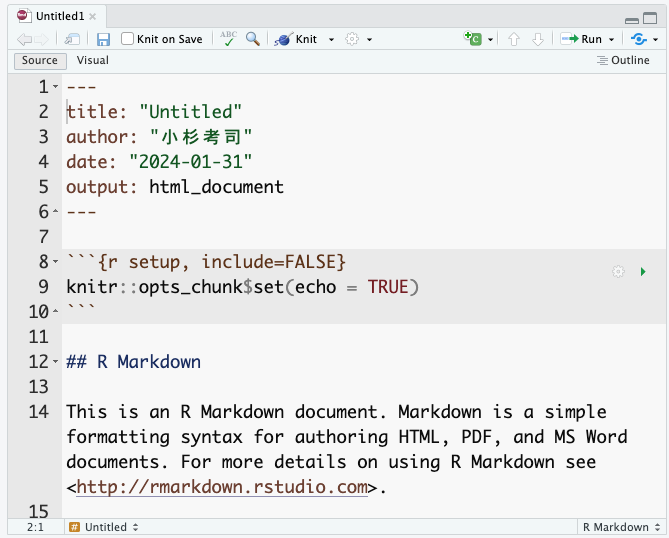
\includegraphics{Figs/04_RmdSample.png}

}

\caption{Rmarkdownファイルのサンプル}

\end{figure}%%
\begin{figure}[H]

{\centering 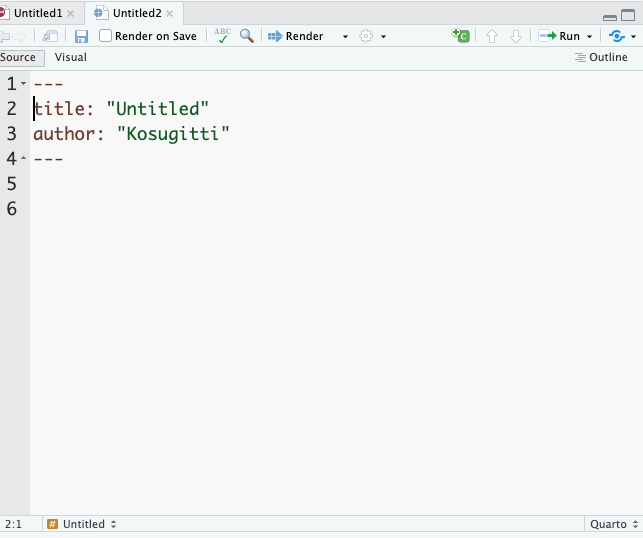
\includegraphics{Figs/04_QmdSample.png}

}

\caption{Quartoファイルのサンプル}

\end{figure}%

Rmarkdown,Quartoともに,ファイルの冒頭に4つのハイフンで囲まれた領域が見て取れるだろう。これはYAML(Yet
Another Markup
Languageの略。ここはまだマークアップ領域じゃないよということ)と呼ばれる,文書全体に対する設定をする領域のことである。

\section{プロットによる基本的な描画}\label{ux30d7ux30edux30c3ux30c8ux306bux3088ux308bux57faux672cux7684ux306aux63cfux753b}

\section{ggplotによる描画}\label{ggplotux306bux3088ux308bux63cfux753b}

\section{各種geomの練習}\label{ux5404ux7a2egeomux306eux7df4ux7fd2}

\section{ggplotオブジェクトを並べる}\label{ggplotux30aaux30d6ux30b8ux30a7ux30afux30c8ux3092ux4e26ux3079ux308b}

\section{テーマの変更(レポートに合わせる)}\label{ux30c6ux30fcux30deux306eux5909ux66f4ux30ecux30ddux30fcux30c8ux306bux5408ux308fux305bux308b}

\section{References}\label{references-3}


\bookmarksetup{startatroot}

\chapter{Rでプログラミング}\label{rux3067ux30d7ux30edux30b0ux30e9ux30dfux30f3ux30b0}

\section{代入}\label{ux4ee3ux5165}

\section{反復}\label{ux53cdux5fa9}

\section{条件分岐}\label{ux6761ux4ef6ux5206ux5c90}

\section{自作関数}\label{ux81eaux4f5cux95a2ux6570}

\section{さまざまな乱数}\label{ux3055ux307eux3056ux307eux306aux4e71ux6570}

\section{確率分布の関数}\label{ux78baux7387ux5206ux5e03ux306eux95a2ux6570}

\section{References}\label{references-4}


\bookmarksetup{startatroot}

\chapter{確率とシミュレーション}\label{ux78baux7387ux3068ux30b7ux30dfux30e5ux30ecux30fcux30b7ux30e7ux30f3}

\section{サンプリング関数}\label{ux30b5ux30f3ux30d7ux30eaux30f3ux30b0ux95a2ux6570}

\section{期待値と分散のシミュレーション}\label{ux671fux5f85ux5024ux3068ux5206ux6563ux306eux30b7ux30dfux30e5ux30ecux30fcux30b7ux30e7ux30f3}

\section{母集団と標本}\label{ux6bcdux96c6ux56e3ux3068ux6a19ux672c}

\section{一致性}\label{ux4e00ux81f4ux6027}

\section{不偏性}\label{ux4e0dux504fux6027}

\section{有効性}\label{ux6709ux52b9ux6027}

\section{References}\label{references-5}


\bookmarksetup{startatroot}

\chapter{統計的仮設検定の論理とエラー}\label{ux7d71ux8a08ux7684ux4eeeux8a2dux691cux5b9aux306eux8ad6ux7406ux3068ux30a8ux30e9ux30fc}

\section{帰無仮説検定の論理}\label{ux5e30ux7121ux4eeeux8aacux691cux5b9aux306eux8ad6ux7406}

\section{相関係数の検定}\label{ux76f8ux95a2ux4fc2ux6570ux306eux691cux5b9a}

\section{標本相関係数の分布}\label{ux6a19ux672cux76f8ux95a2ux4fc2ux6570ux306eux5206ux5e03}

\section{2種類の検定のエラー確率}\label{ux7a2eux985eux306eux691cux5b9aux306eux30a8ux30e9ux30fcux78baux7387}

\section{References}\label{references-6}


\bookmarksetup{startatroot}

\chapter{平均値差の検定}\label{ux5e73ux5747ux5024ux5deeux306eux691cux5b9a}

\section{一標本検定}\label{ux4e00ux6a19ux672cux691cux5b9a}

\section{二標本検定}\label{ux4e8cux6a19ux672cux691cux5b9a}

\section{二標本検定(ウェルチの補正)}\label{ux4e8cux6a19ux672cux691cux5b9aux30a6ux30a7ux30ebux30c1ux306eux88dcux6b63}

\section{対応のある二標本検定}\label{ux5bfeux5fdcux306eux3042ux308bux4e8cux6a19ux672cux691cux5b9a}

\section{レポートを書くような課題}\label{ux30ecux30ddux30fcux30c8ux3092ux66f8ux304fux3088ux3046ux306aux8ab2ux984c}

\section{References}\label{references-7}


\bookmarksetup{startatroot}

\chapter{多群の平均値差の検定}\label{ux591aux7fa4ux306eux5e73ux5747ux5024ux5deeux306eux691cux5b9a}

\section{分散分析の基礎}\label{ux5206ux6563ux5206ux6790ux306eux57faux790e}

\section{検定の多重性}\label{ux691cux5b9aux306eux591aux91cdux6027}

\section{ANOVA君を使う}\label{anovaux541bux3092ux4f7fux3046}

\section{Betweenデザイン}\label{betweenux30c7ux30b6ux30a4ux30f3}

\section{Withinデザイン}\label{withinux30c7ux30b6ux30a4ux30f3}

\section{References}\label{references-8}


\bookmarksetup{startatroot}

\chapter{帰無仮説検定のシミュレーション}\label{ux5e30ux7121ux4eeeux8aacux691cux5b9aux306eux30b7ux30dfux30e5ux30ecux30fcux30b7ux30e7ux30f3}

\section{統計的検定とQRPs}\label{ux7d71ux8a08ux7684ux691cux5b9aux3068qrps}

\section{タイプ2エラー確率のコントールとサンプルサイズ設計}\label{ux30bfux30a4ux30d7uxff12ux30a8ux30e9ux30fcux78baux7387ux306eux30b3ux30f3ux30c8ux30fcux30ebux3068ux30b5ux30f3ux30d7ux30ebux30b5ux30a4ux30baux8a2dux8a08}

\section{サンプルサイズ設計の実践}\label{ux30b5ux30f3ux30d7ux30ebux30b5ux30a4ux30baux8a2dux8a08ux306eux5b9fux8df5}

\subsection{一標本t検定}\label{ux4e00ux6a19ux672ctux691cux5b9a}

\subsection{二標本t検定}\label{ux4e8cux6a19ux672ctux691cux5b9a}

\subsection{相関係数のサンプルサイズ設計}\label{ux76f8ux95a2ux4fc2ux6570ux306eux30b5ux30f3ux30d7ux30ebux30b5ux30a4ux30baux8a2dux8a08}

\section{References}\label{references-9}


\bookmarksetup{startatroot}

\chapter{回帰分析}\label{ux56deux5e30ux5206ux6790}

\section{回帰分析の基礎}\label{ux56deux5e30ux5206ux6790ux306eux57faux790e}

\section{重回帰分析の場合}\label{ux91cdux56deux5e30ux5206ux6790ux306eux5834ux5408}

\section{回帰分析のいくつかの特徴}\label{ux56deux5e30ux5206ux6790ux306eux3044ux304fux3064ux304bux306eux7279ux5fb4}

\section{シミュレーションとパラメタリカバリ}\label{ux30b7ux30dfux30e5ux30ecux30fcux30b7ux30e7ux30f3ux3068ux30d1ux30e9ux30e1ux30bfux30eaux30abux30d0ux30ea}

\section{係数の標準誤差}\label{ux4fc2ux6570ux306eux6a19ux6e96ux8aa4ux5dee}

\section{係数の検定}\label{ux4fc2ux6570ux306eux691cux5b9a}

\section{サンプルサイズ設計}\label{ux30b5ux30f3ux30d7ux30ebux30b5ux30a4ux30baux8a2dux8a08}

\section{References}\label{references-10}


\bookmarksetup{startatroot}

\chapter{線型モデルの展開}\label{ux7ddaux578bux30e2ux30c7ux30ebux306eux5c55ux958b}

\section{一般線型モデル}\label{ux4e00ux822cux7ddaux578bux30e2ux30c7ux30eb}

\section{一般化線型モデル}\label{ux4e00ux822cux5316ux7ddaux578bux30e2ux30c7ux30eb}

\section{階層線型モデル}\label{ux968eux5c64ux7ddaux578bux30e2ux30c7ux30eb}

\section{References}\label{references-11}


\bookmarksetup{startatroot}

\chapter{多変量解析の入り口}\label{ux591aux5909ux91cfux89e3ux6790ux306eux5165ux308aux53e3}

\section{因子分析}\label{ux56e0ux5b50ux5206ux6790}

\section{構造方程式モデリング}\label{ux69cbux9020ux65b9ux7a0bux5f0fux30e2ux30c7ux30eaux30f3ux30b0}

\section{References}\label{references-12}



\printbibliography[title=引用文献]


\end{document}
